\documentclass{article}

\usepackage[utf8]{inputenc}
\usepackage[pdftex]{graphicx}
\usepackage[left=3cm,right=3cm,top=3cm,bottom=3cm]{geometry}
\usepackage[T1]{fontenc}
\usepackage[francais,english]{babel}
\frenchbsetup{StandardLists=true}
\selectlanguage{english}


\usepackage{amsmath}
\usepackage{amssymb}
\usepackage{mathtools}
\usepackage{slashbox}


\usepackage{caption}
\usepackage[hidelinks]{hyperref}
\usepackage{xcolor}


%ALGORITHM
\usepackage{algorithm}
\usepackage[noend]{algpseudocode}
\renewcommand{\algorithmicforall}{\textbf{for each}}
\newcommand{\var}[1]{\mathit{#1}}
\newcommand{\func}[1]{\mathrm{#1}}
\algdef{SE}[DOWHILE]{Do}{doWhile}{\algorithmicdo}[1]{\algorithmicwhile\ #1}
%

\usepackage{listings}

\usepackage{graphicx}

\renewcommand\thesection{\arabic{section}}

\usepackage{fancyhdr}
\pagestyle{fancy}
\fancyhf{}
\fancyhead[R]{\thepage}


\title{[INFO-F409] Learning Dynamics \\ Third assignment}
\author{\bsc{BUI QUANG PHUONG} Quang Linh \\ Université libre de Bruxelles - ULB ID : 000427796  \\ MA1 Computer Sciences}
\date{December 2018}

\begin{document}

\maketitle

\tableofcontents

\newpage
\section{First game: N-Armed Bandit}

\subsection*{Context}
The first game that we discuss is the N-Armed Bandit game. In this problem, the player has the choice between 4 actions (i.e 4 arms) which give for each action a different reward calculated according to the reward distribution table presented in \autoref{fig:action-table} \footnote{My ULB enrolment number is 000427796 and is then ending by a 6. The table selected is then the Table 4 in the statement}. The rewards are subject to noise according to a normal probability distribution with mean $Q^{*}_{ai}$ and standard deviation $\sigma_{i}$. The results presented for this game in the document are based on \textbf{1000 simulations}. 

\begin{figure}[H]
  \centering
  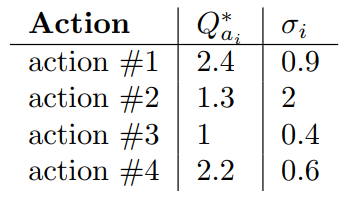
\includegraphics[scale=0.4]{fig/action-table.png}
  \caption{Reward distributions for each action}
  \label{fig:action-table}
\end{figure}


\subsection{Exercise 1}

\subsubsection*{Statement}
\textit{Run the algorithms and provide the requested plots. Comment the results. Which algorithms arrive close to the best arm after 1000 iterations? Which one arrives there faster? Explain your findings.} 

\subsubsection{Average reward according to the algorithm}

The \autoref{fig:bandit-avgReward} shows the average reward earned for each algorithm used. The figure is proving that picking the action randomly is the worst choice to optimise the reward while using the $\epsilon$-Greedy strategy with an $\epsilon$ value of 0 is the best choice. Indeed, $\epsilon = 0$ means that the player is \textbf{always} selecting the arm with the potential best reward. Here, the best arm has a reward of 2.4. The average reward by using this strategy is then approaching this value. 

\begin{figure}[H]
  \centering
  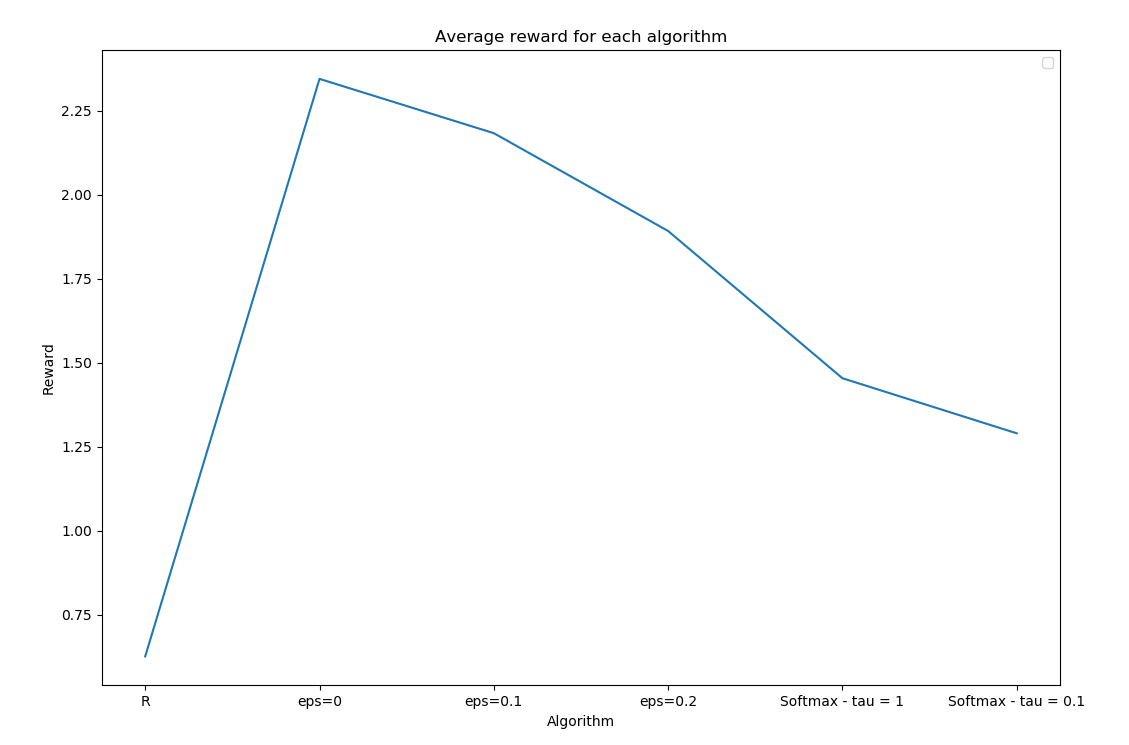
\includegraphics[scale=0.32]{fig/bandit-avgReward.png}
  \caption{Average reward for each algorithm}
  \label{fig:bandit-avgReward}
\end{figure}

\subsubsection{Evolution of the Q-value for each arm}

The evolution of the $Q$ matrix along time by using the different strategy are shown in the \autoref{fig:bandit-arm1} for the first arm, \autoref{fig:bandit-arm2} for the second arm, \autoref{fig:bandit-arm3} for third arm and \autoref{fig:bandit-arm4} for the fourth arm. We remind that these results are obtained by running the simulation 1000 times. What we can observe from the results is that the general behaviour of each algorithm for each arm is that the Q-values are converging to the average payoff\footnote{see \autoref{fig:action-table}} of the arm. Moreover, we see that the evolution of the Q-values for the first arm is quite more steady than others. This can be explained because all the algorithms tend to take the optimal action, i.e the action with the best average payoff (action 1 with a payoff of 2.4). Now let's analyse the result for each arm one by one.  \\

\noindent 
\textbf{Arm 1:}  In this case, no matter which strategy you chose, all the Q-values seem to converge to the average reward of 2.4. A stationary state can be found after 100-150 simulations. At this time the values variate less and begin to be steady. As explained before, this trend is due to the fact that the first arm is in average the best action to pick. \\

\noindent 
\textbf{Arm 2, 3 and 4:} Concerning the other arms, what we observe is that the Softmax algorithm with $\tau = 0.1$ has a constant null estimation of Q-values. To explain such a quirk, we need to explain what does $\tau$ means in the Softmax algorithm. $\tau$ is defined by what we call the \textit{computational temperature}. This feature means that for a high temperature ($\rightarrow \infty$), all actions have nearly the same probability while for a low temperature ($\rightarrow 0$), the action with the best average/expected reward has nearly a probability of 1 to be selected. In our case, when $\tau = 0.1$, it means that the temperature is really low. Therefore, the action with the best expected payoff, i.e action 1, has a probability of 1. Thus, it explains why for every other arms than arm 1, the evaluation of the Q-values for the Softmax algorithm with $tau = 0.1$ is equals to zero. Concerning the other algorithms, their behaviour is quite similar to Arm 1, the Q-values are evolving such that they tend to converge to the average reward of the arm despite they are more variables. Their stationary state is then later than for Arm 1 (i.e 200-250 simulations for Arm 2, 400-450 simulations for Arm 3 and 500-550 for Arm 4). \\

\noindent
\textbf{In summary, what are the differences between each algorithm ?} The algorithms are separated into two categories : the random and the greedy actions. The first one is simply selecting the action for each simulation randomly. The efficiency of this algorithm is somehow bad. It would chose the optimal action with a probability of 1/4. On the second hand, we have the greedy actions. The meaning of this type of actions is that you are \textbf{exploiting} your current knowledge of the values of the actions while if you are playing randomly, then non-greedy, you are \textbf{exploring} the environment. The goal of playing greedy is to improve along time your action's choice from your previous actions. Thus, exploitation is the good method to adopt to optimize your choice. However, one drawback is that when it explores it chooses equally among all actions. This means that it is as likely to choose the action with the worst expected reward as it is to choose the action with the best expected reward. In the case where the worst actions are very bad, this may be unsatisfactory. The solution of this is given by the Softmax algorithm which gives a higher probability to the best actions and a lower probability to the bad actions. This algorithm is characterized by $\tau$, the computational temperature. As said before, this feature spreads the probabilities equally or not according to the value of $\tau$. The probabilities are computed following this formula : 

$$ \frac{e^{\frac{Q_{t}(a)}{\tau}}}{\sum_{b=1}^{n} e^{\frac{Q_{t}(a)}{\tau}}} $$    

where $a$ is the action to play, $n$ the number of actions and $\tau$ the computational temperature. 


\begin{figure}[H]
  \centering
  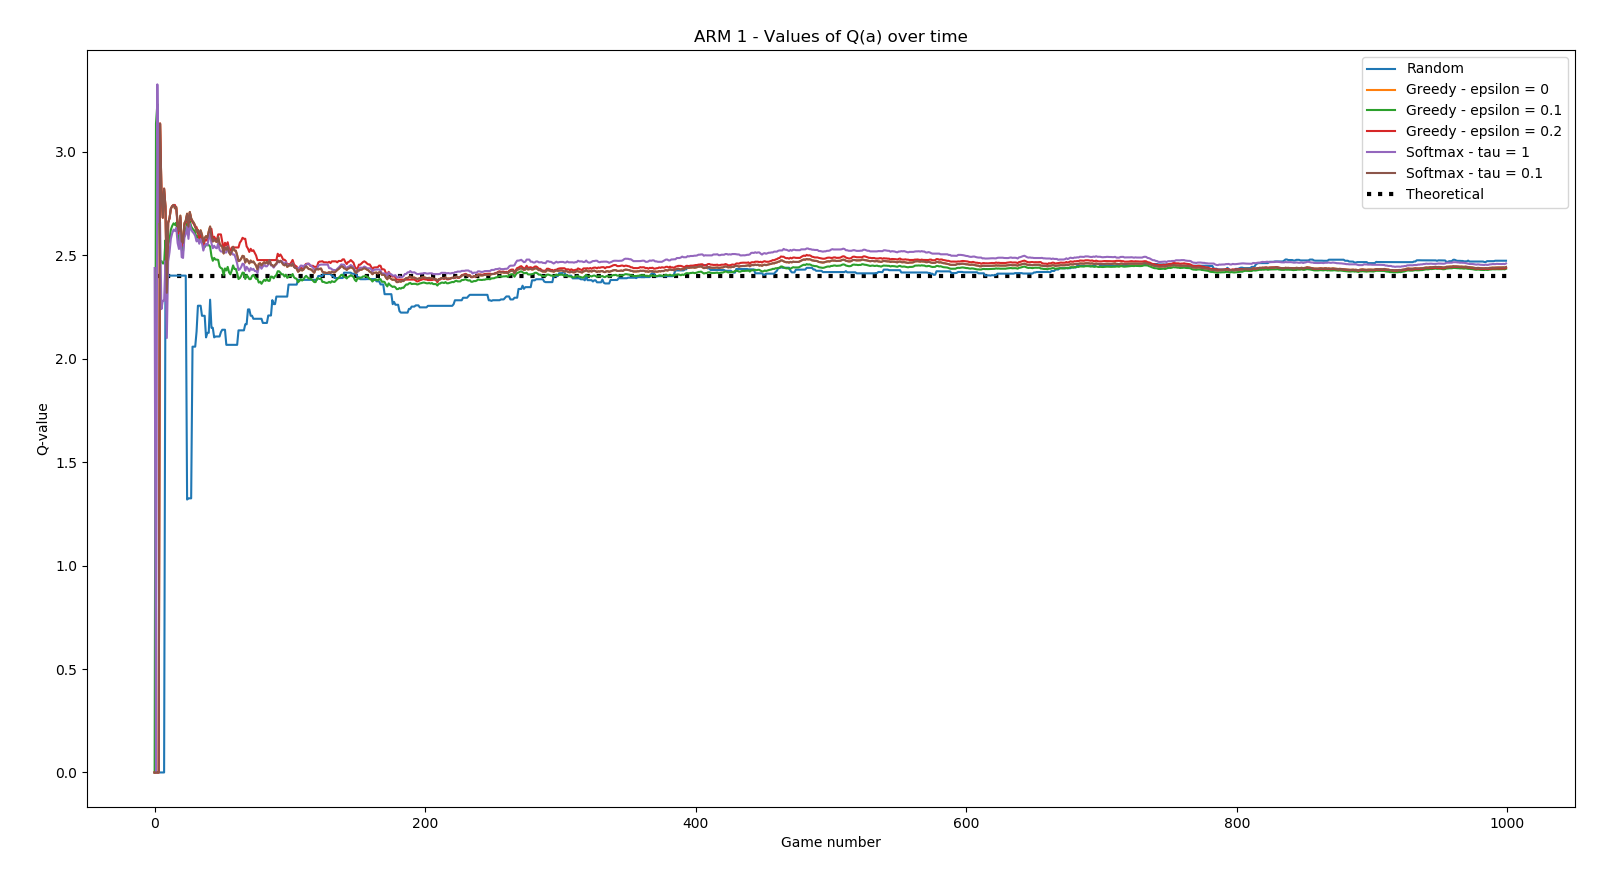
\includegraphics[scale=0.35]{fig/bandit-arm1.png}
  \caption{Evolution of the Q-value for Arm 1}
  \label{fig:bandit-arm1}
\end{figure}

\begin{figure}[H]
  \centering
  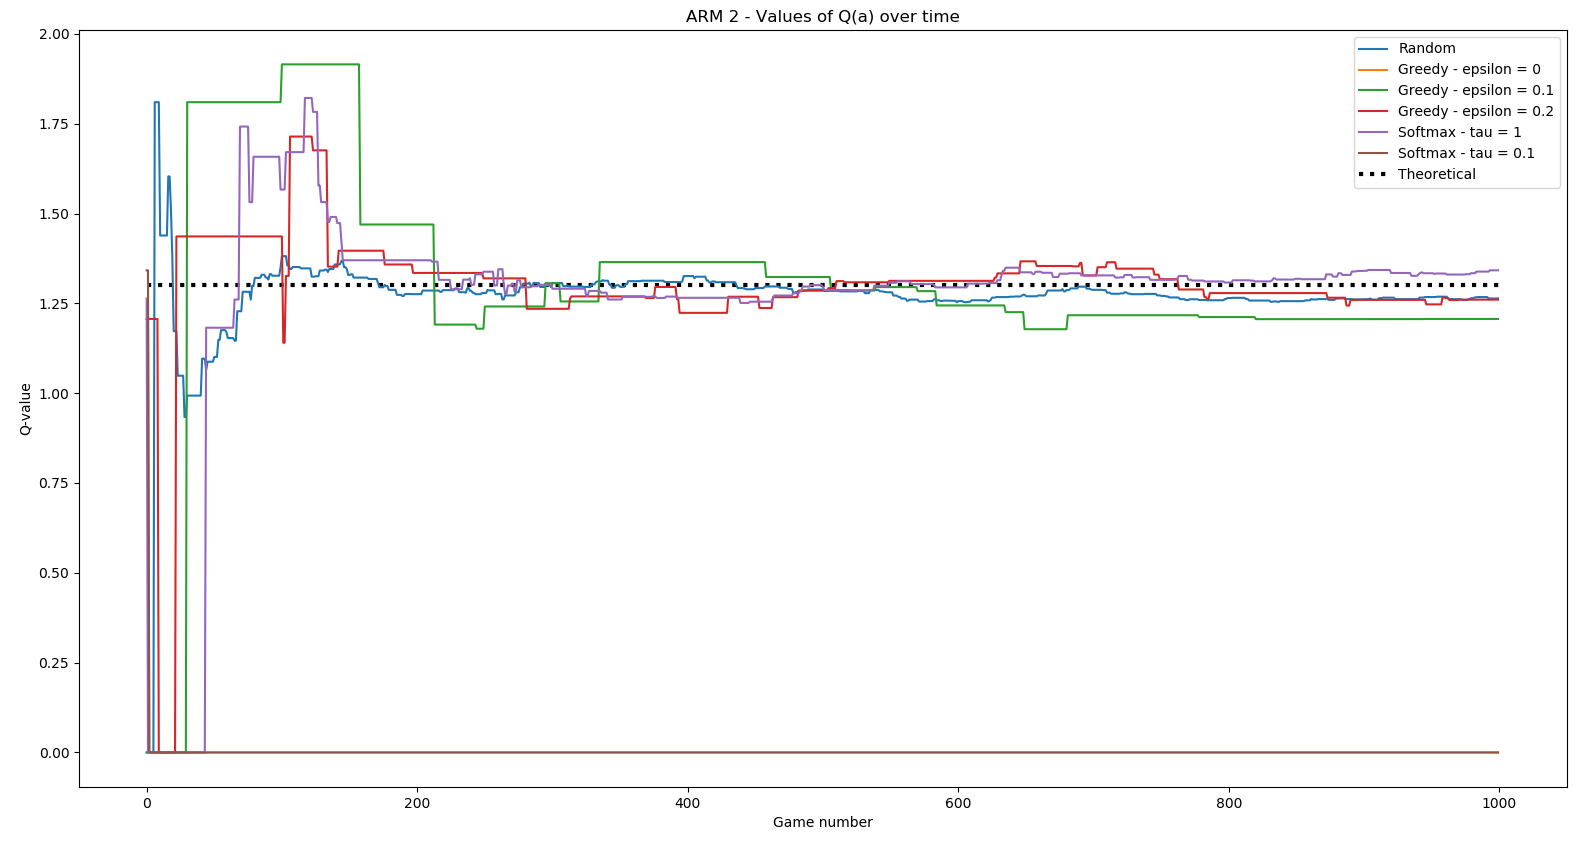
\includegraphics[scale=0.35]{fig/bandit-arm2.png}
  \caption{Evolution of the Q-value for Arm 2}
  \label{fig:bandit-arm2}
\end{figure}

\begin{figure}[H]
  \centering
  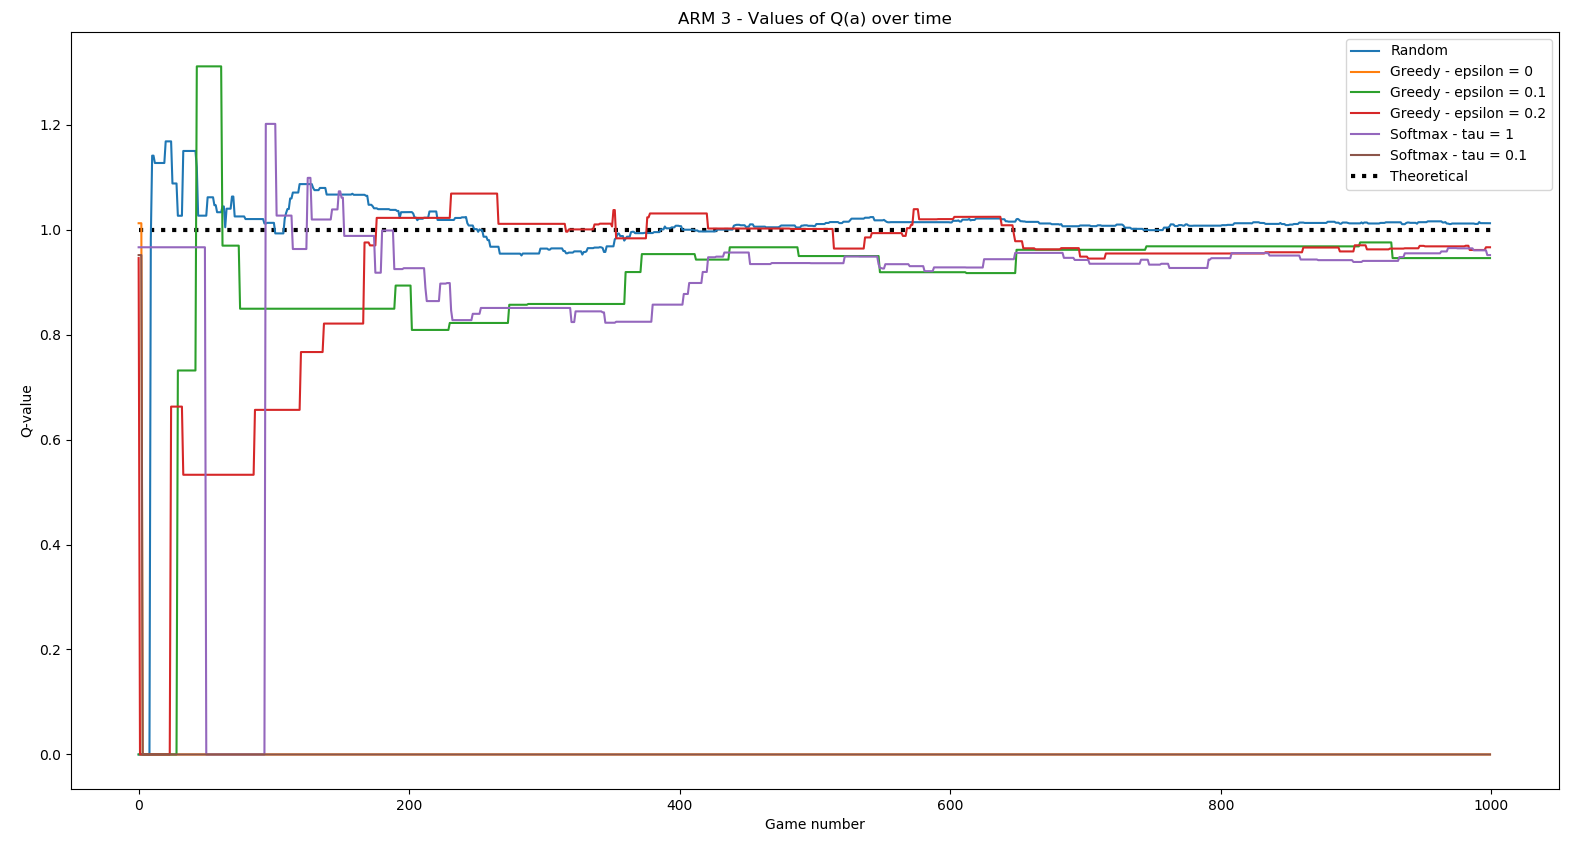
\includegraphics[scale=0.35]{fig/bandit-arm3.png}
  \caption{Evolution of the Q-value for Arm 3}
  \label{fig:bandit-arm3}
\end{figure}

\begin{figure}[H]
  \centering
  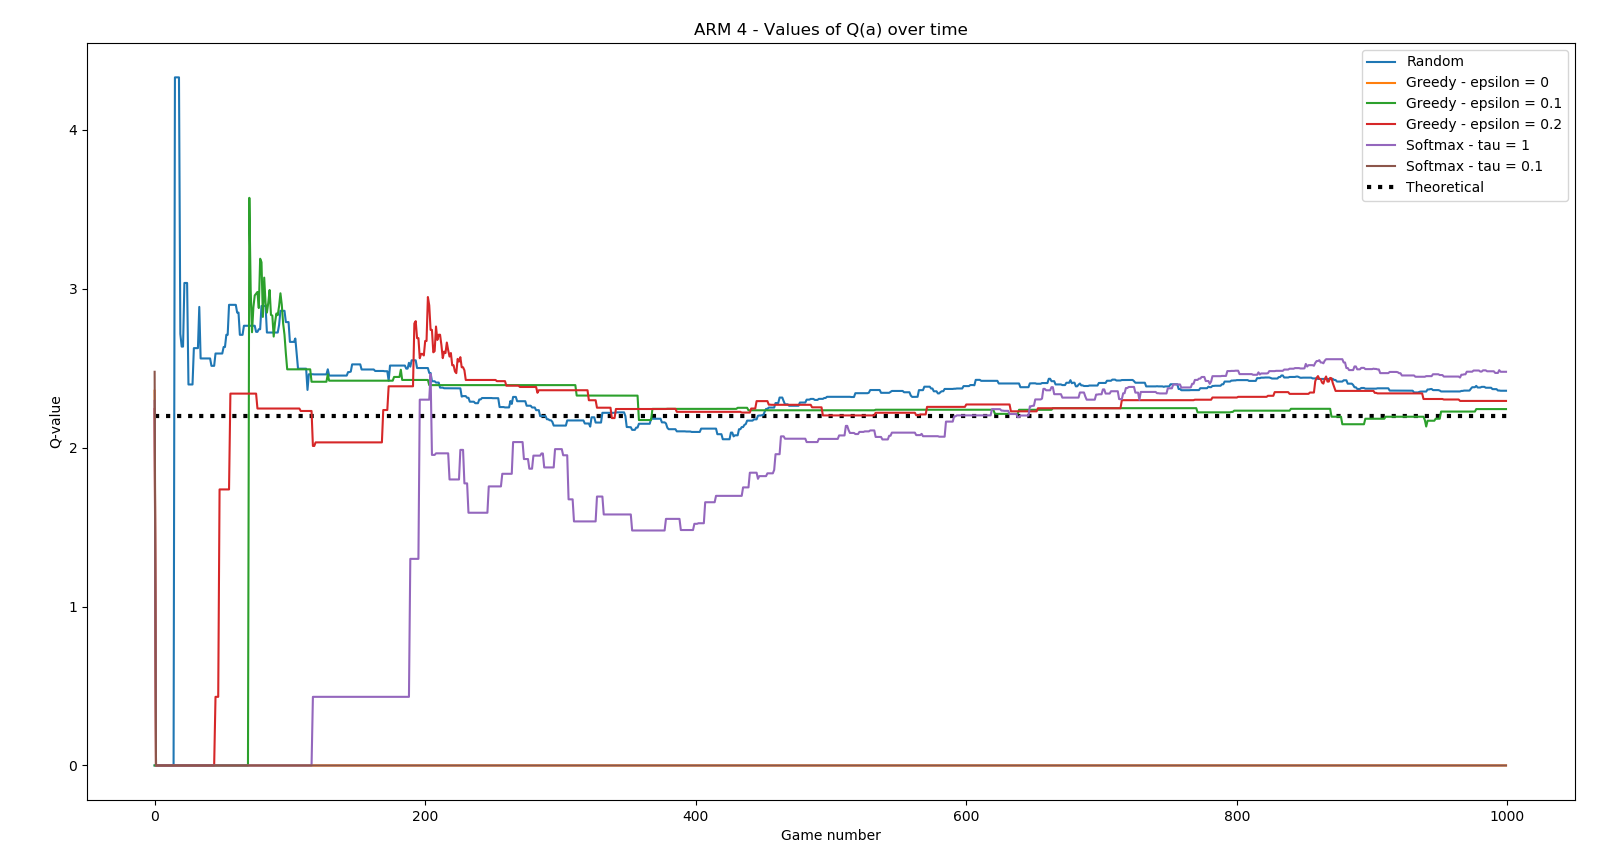
\includegraphics[scale=0.35]{fig/bandit-arm4.png}
  \caption{Evolution of the Q-value for Arm 4}
  \label{fig:bandit-arm4}
\end{figure}

\newpage
\subsubsection{Frequency of each action being selected}

The number of times that an action is selected on 1000 simulations for every algorithm is shown in the \autoref{fig:bandit-counters}. In the first row from left to right, the algorithms represented are Random, Greedy with $\epsilon = 0$, Greedy with $\epsilon = 0.1$, in the second row, Greedy with $\epsilon = 0.2$, Softmax with $\tau = 1$ and Softmax with $\tau = 0.1$. For the random strategy, we observe that the selecting rate of each action is somehow equivalent while for the other strategies, the first action is hardly dominating the other actions. In summary, this is mainly due to the fact that all the strategies except the random one is tending to select the best action. This is explained in details in the previous section. 

\begin{figure}[H]
  \centering
  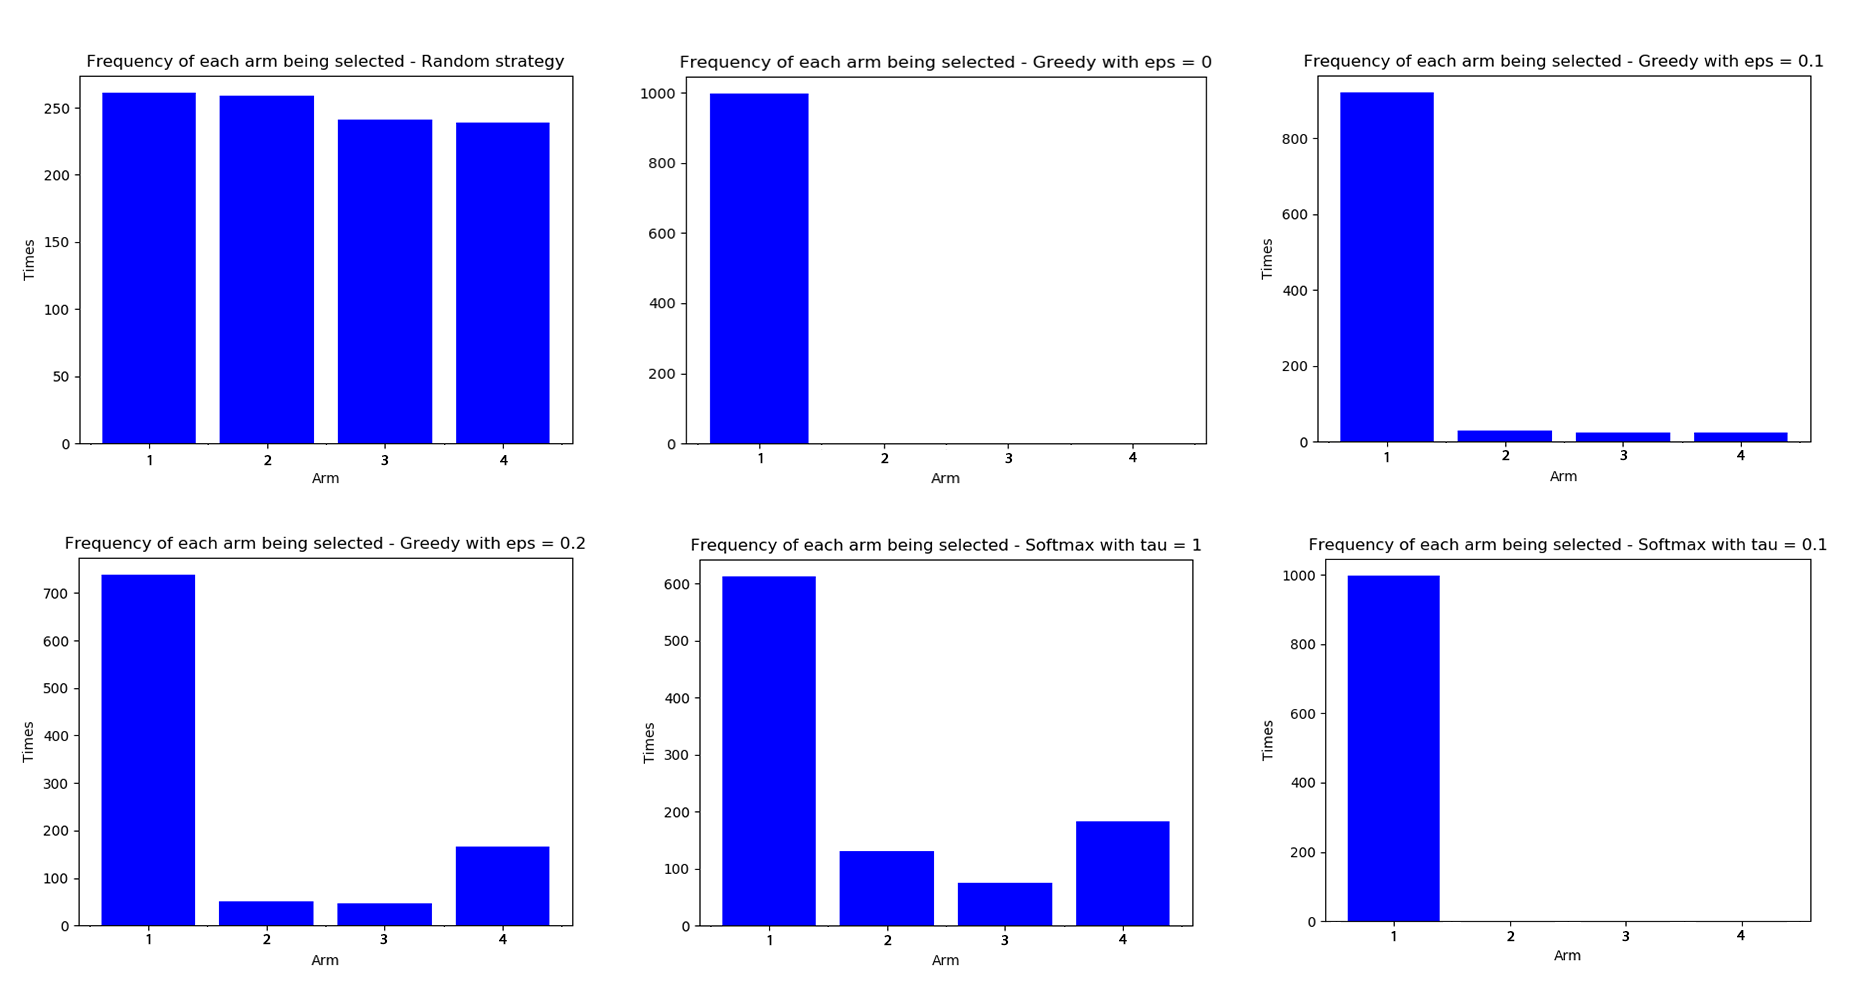
\includegraphics[scale=1]{fig/bandit-counters.png}
  \caption{Frequency of each arm being selected for 1000 time steps}
  \label{fig:bandit-counters}
\end{figure}

\subsection{Exercise 2}

\subsubsection*{Statement}
\textit{Re-run Exercise 1 doubling the standard deviations of each arm, and comment the plots and results. Discuss the results. Is this problem harder or easier to learn? Does the performance of the algorithms change significantly? Which of the above performs best now?} 

\subsubsection{Average reward according to the algorithm}
The graph obtained for the average reward for each algorithm has the same appearance than \autoref{fig:bandit-avgReward}. Modifying the value of the standard deviation has apparently no real impact on the graph. 

\begin{figure}[H]
  \centering
  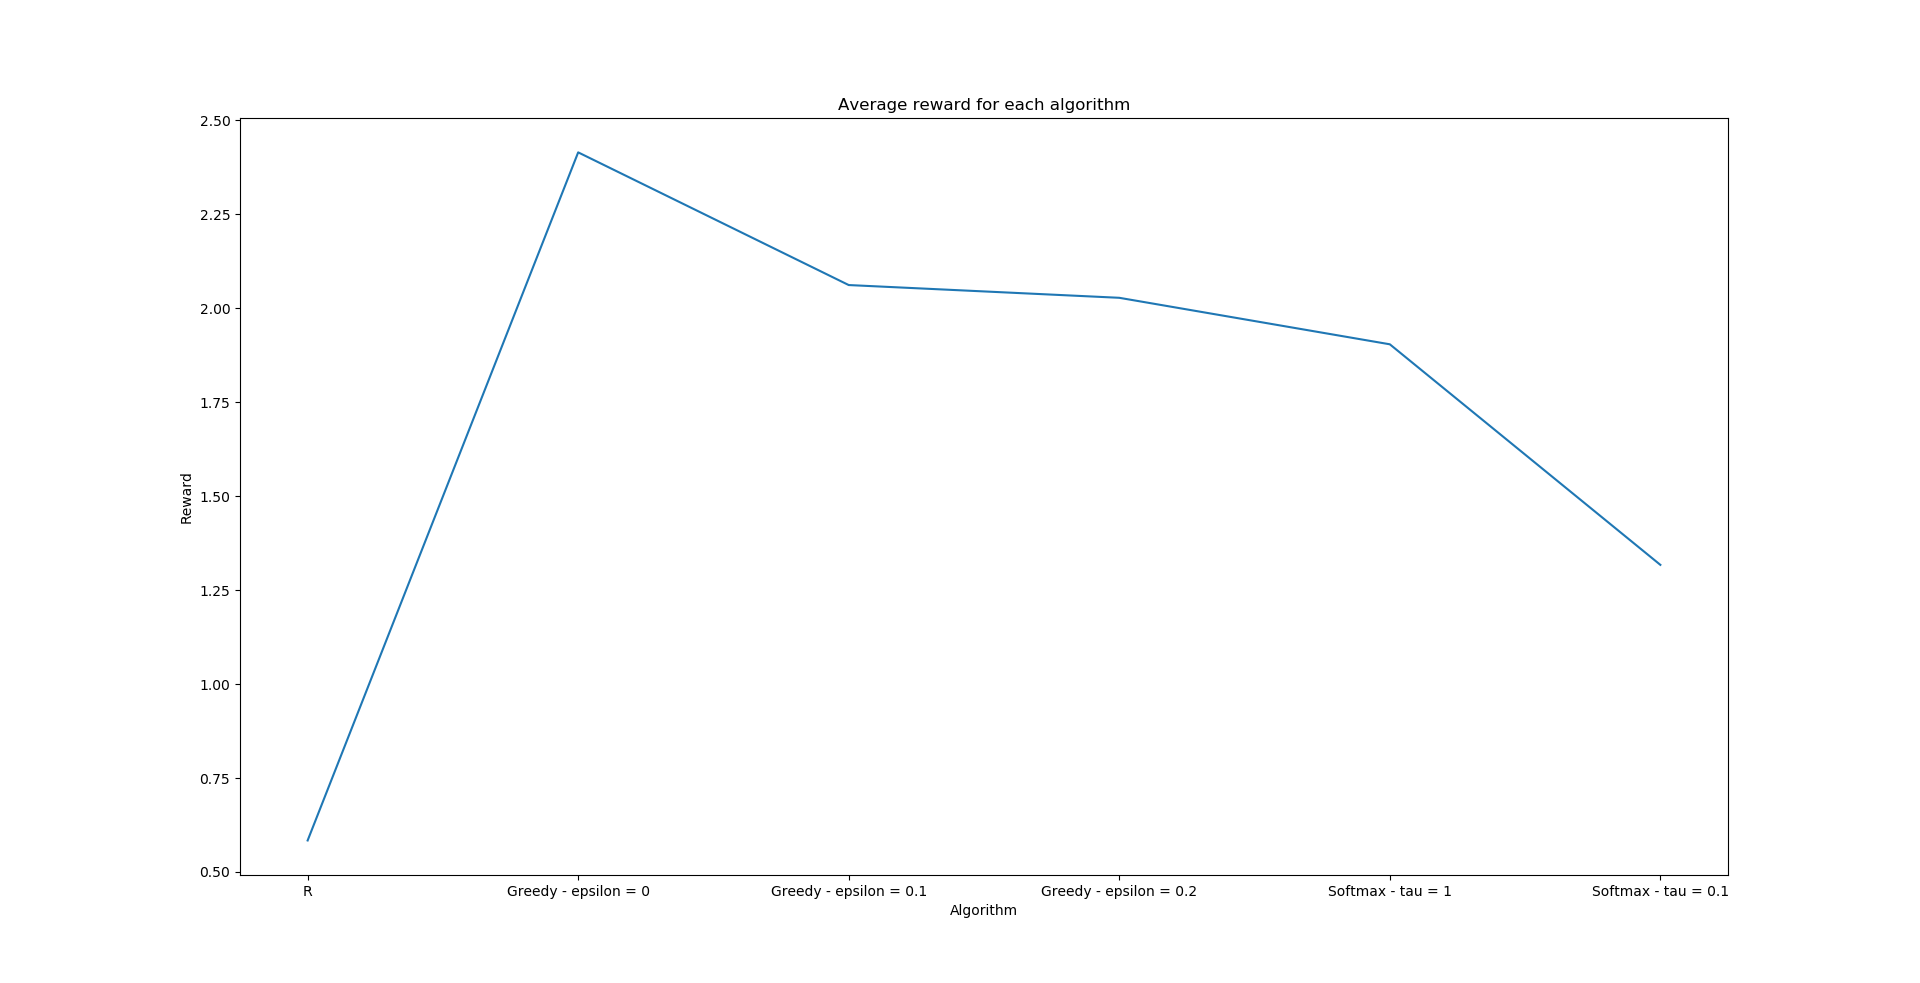
\includegraphics[scale=0.3]{fig/bandit2-avgReward.png}
  \caption{Average reward for each algorithm with 2$\sigma$}
  \label{fig:bandit2-avgReward}
\end{figure}

\subsubsection{Evolution of the Q-value for each arm}
Doubling the standard deviation means that the noise is 2 times bigger. In theory, the results at the end of the 1000 simulations should be the same because the mean has not been modified. Nevertheless, at the beginning the values should be more noisy and should take more time to find the mean value. It's exactly what we can observe from the results presented in the figures. At the end of the 1000 simulations, the values are somehow the same, they are all converging to the corresponding expected reward of the arm. However, the stationary state is reached a bit later compared to the figures obtained before doubling the value of $\sigma$. For instance, the evolution of the Q-value for the first arm is really noisy at the beginning and is reaching a stationary state near the 350-400th simulation while it was reached before towards 100-150 simulations. 


\begin{figure}[H]
  \centering
  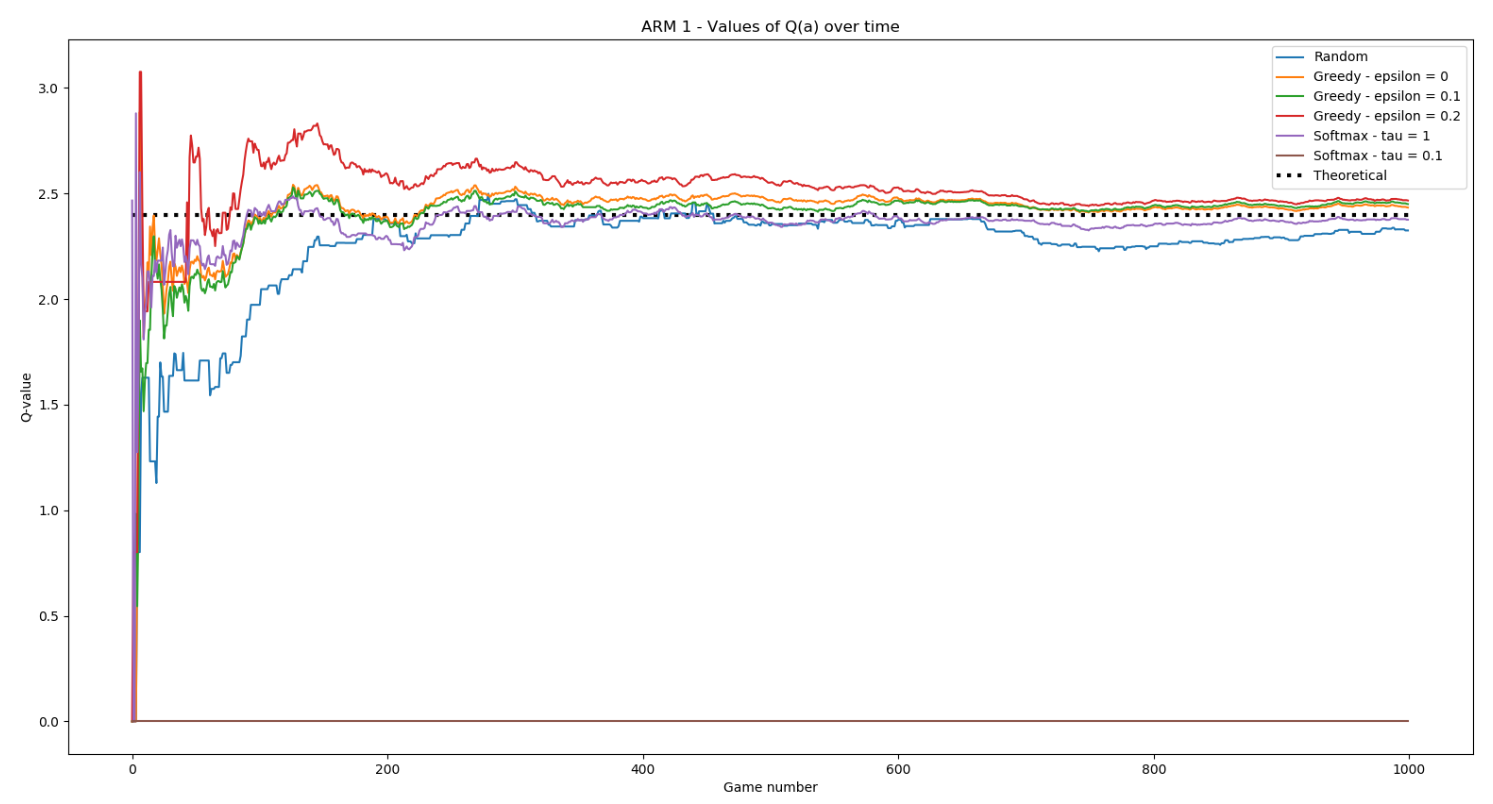
\includegraphics[scale=0.35]{fig/bandit2-arm1.png}
  \caption{Evolution of the Q-value for Arm 1 with 2$\sigma$}
  \label{fig:bandit2-arm1}
\end{figure}

\begin{figure}[H]
  \centering
  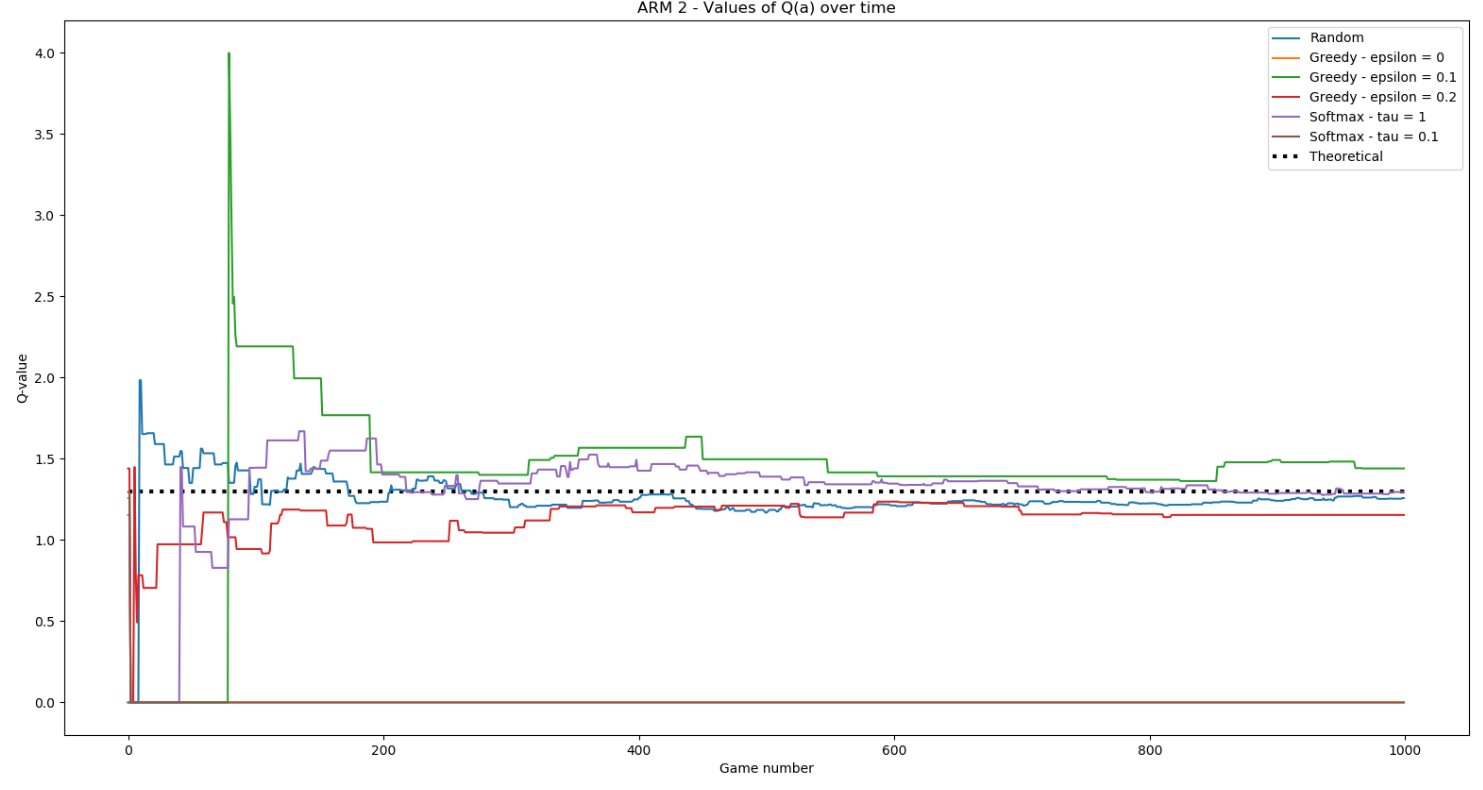
\includegraphics[scale=0.37]{fig/bandit2-arm2.png}
  \caption{Evolution of the Q-value for Arm 2 with 2$\sigma$}
  \label{fig:bandit2-arm2}
\end{figure}

\begin{figure}[H]
  \centering
  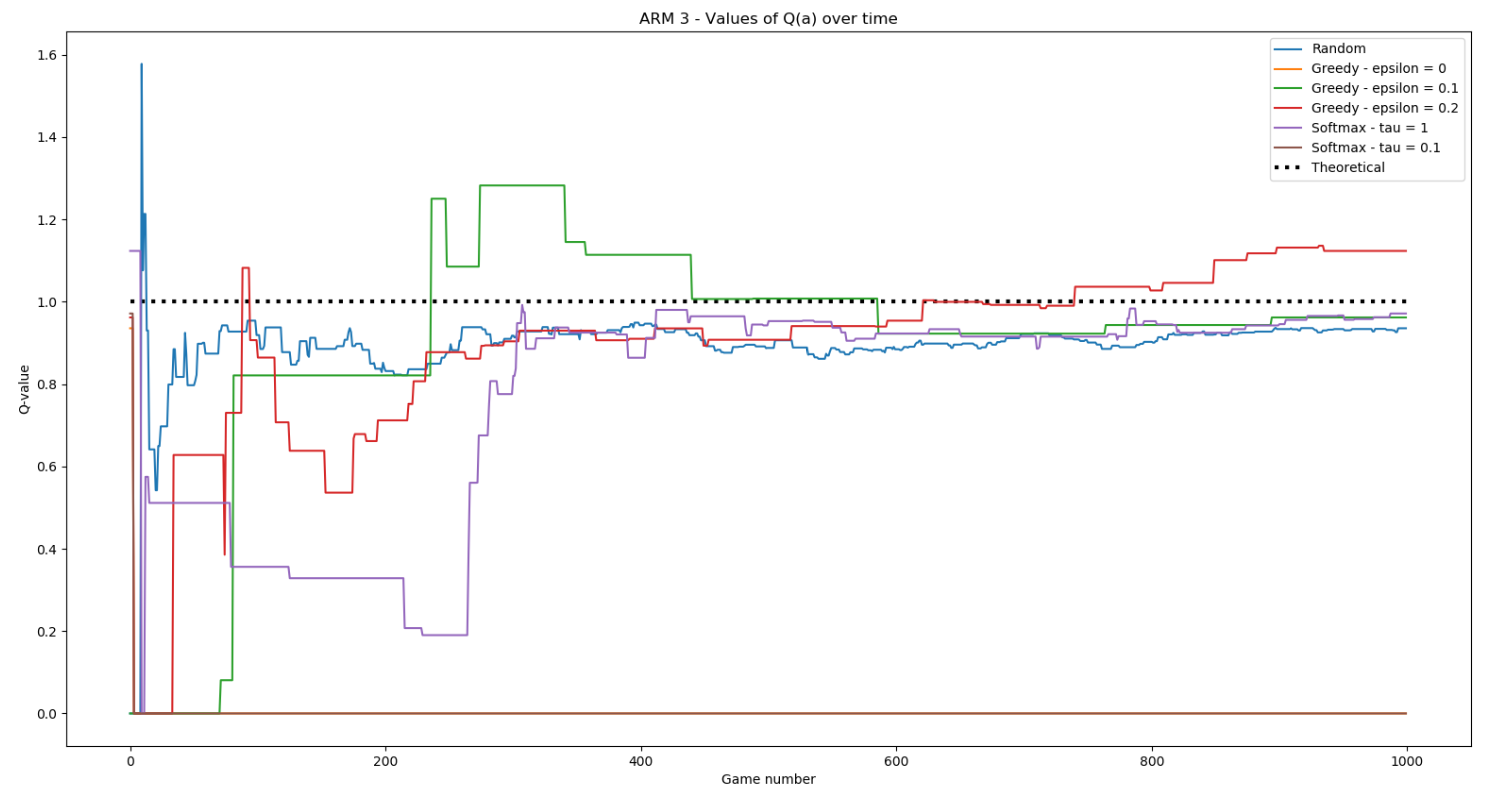
\includegraphics[scale=0.37]{fig/bandit2-arm3.png}
  \caption{Evolution of the Q-value for Arm 3 with 2$\sigma$}
  \label{fig:bandit2-arm3}
\end{figure}

\begin{figure}[H]
  \centering
  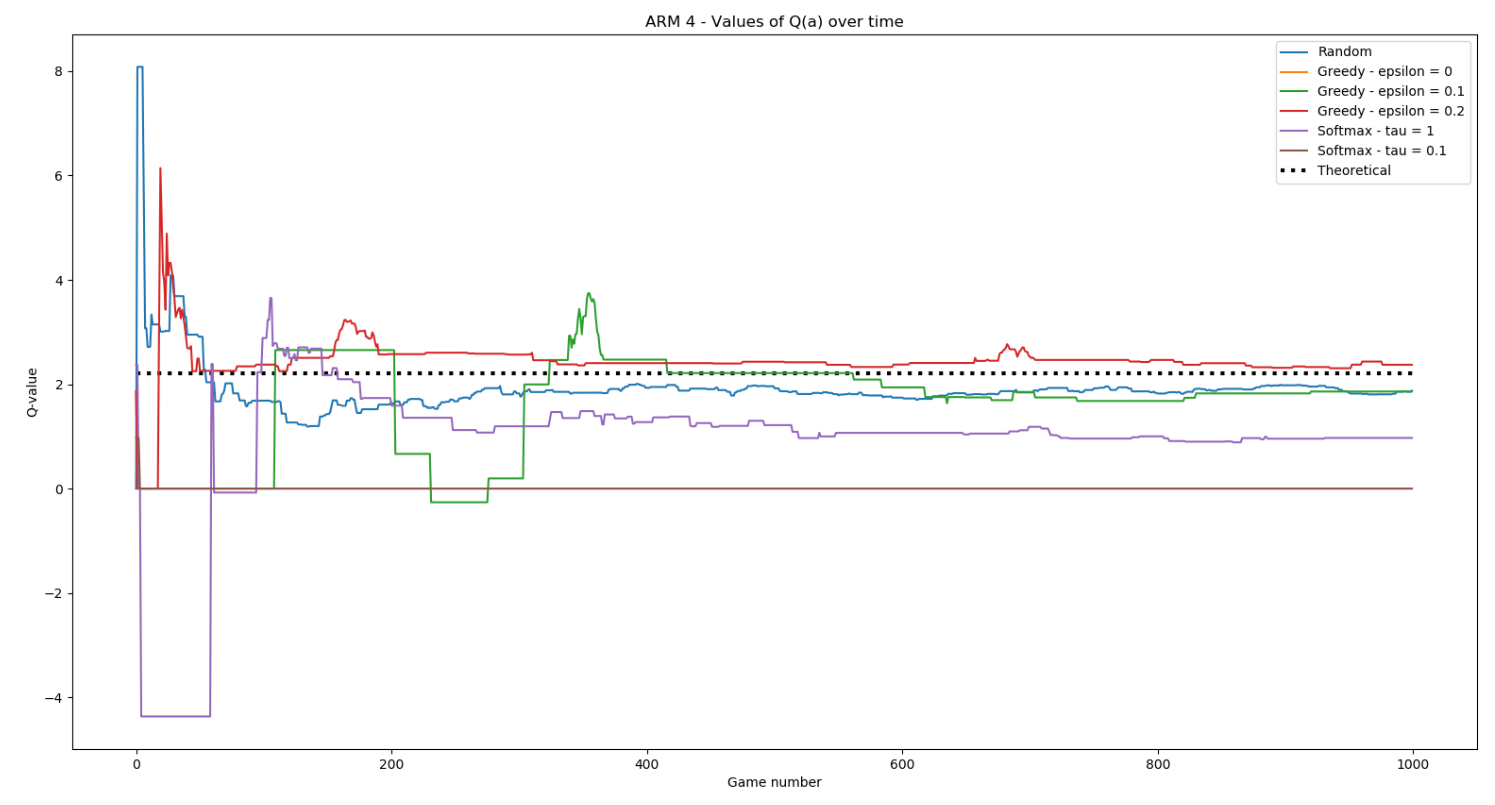
\includegraphics[scale=0.34]{fig/bandit2-arm4.png}
  \caption{Evolution of the Q-value for Arm 4 with 2$\sigma$}
  \label{fig:bandit2-arm4}
\end{figure}

\subsubsection{Frequency of each action being selected}
The general observation in these results is that they really look the same as \autoref{fig:bandit-counters}. However, we can see that for the frequencies of the greedy strategies $> 0$ the actions 2, 3 and 4 are being selected a bit more than \autoref{fig:bandit-counters}. This shows one more time that the noise is more present which means that it takes more simulations to reach the average reward. To summarize, doubling the standard deviation is decreasing the simplicity to learn because of the noise augmentation despite the performance is not changing significantly. Nevertheless, keeping the initial standard deviation is still the best choice to perform the best.    

\begin{figure}[H]
  \centering
  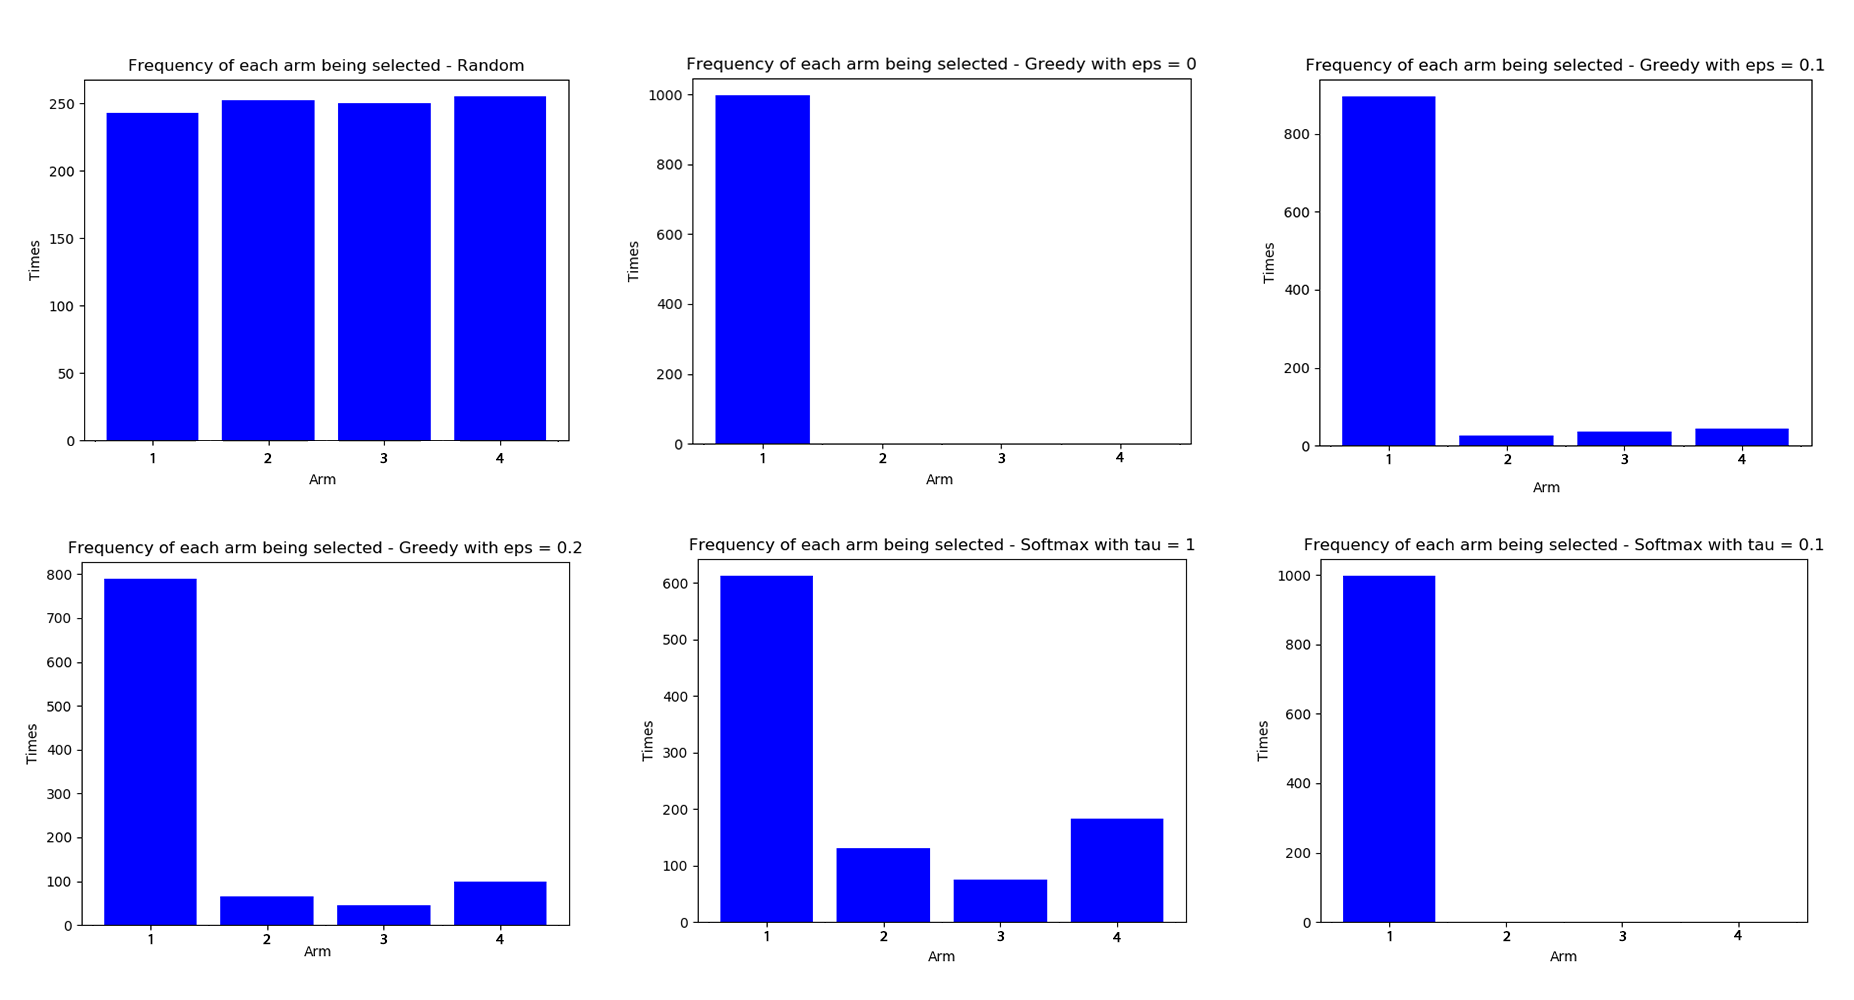
\includegraphics[scale=1]{fig/bandit2-counters.png}
  \caption{Frequency of each arm being selected for 1000 time steps with 2$\sigma$}
  \label{fig:bandit2-counters}
\end{figure}

\subsection{Exercise 3}

\subsubsection*{Statement}
\textit{Re-run exercise 1 with two additional algorithms, and plot their results. The new algorithms have a time-varying parameter, which depends on the iteration number $t = 1, . . . , 1000$. Discuss the results. Are these algorithms better than the ones with a fixed parameter?} 

\subsubsection{Average reward according to the algorithm}

In this section, we are using two new algorithms to run our simulations. These two algorithms are using time-varying parameters : 
\begin{itemize}
\item $\epsilon$-Greedy with parameter $\epsilon = \frac{1}{\sqrt{t}}$ 
\item Softmax with parameter $\tau = 4 \cdot \frac{1000-t}{1000}$
\end{itemize}
such that $t$ is the current simulation time. \\

The two additional algorithms, even the $\epsilon$-Greedy with $\epsilon = \frac{1}{\sqrt{t}}$ or the softmax strategy with $\tau = 4 \cdot \frac{1000-t}{1000}$ seem to be really efficient. Indeed, their average reward is approaching a lot the optimal expected reward.  

\begin{figure}[H]
  \centering
  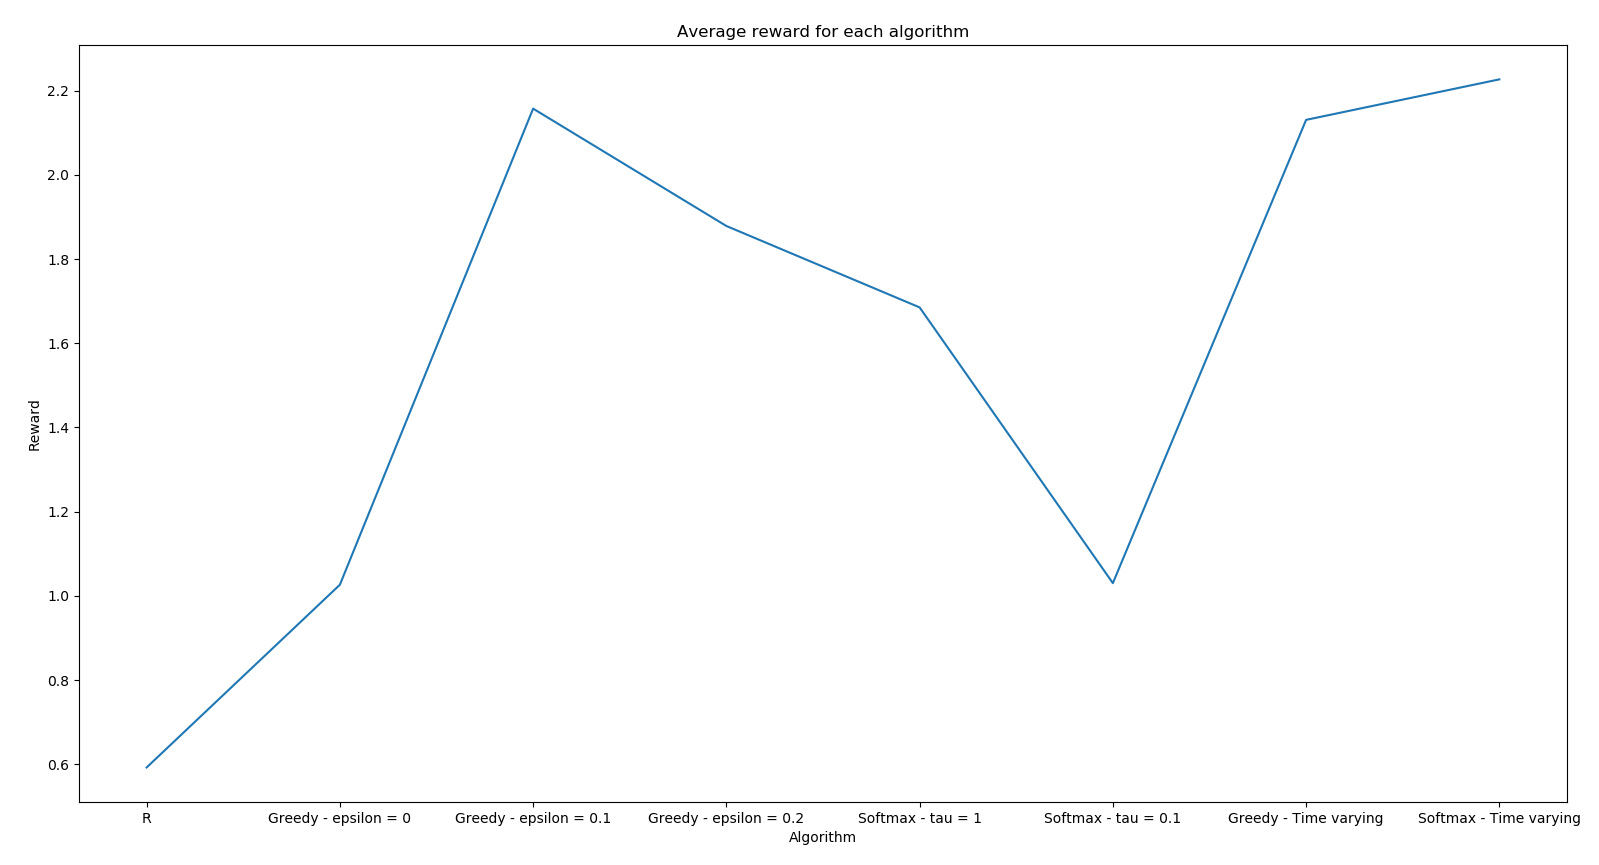
\includegraphics[scale=0.3]{fig/bandit3-avgReward.png}
  \caption{Average reward for each algorithm}
  \label{fig:bandit3-avgReward}
\end{figure}


\subsubsection{Evolution of the Q-value for each arm}

In the following figures, what we can observe from the new algorithms is that the result are quite similar than using these algorithms with fixed parameter. In general, they look somehow steady and their noise level, i.e exploration time, is not really huge. Indeed, their stationary level for the first arm for instance is around 100 rounds as using the fixed parameter. However, what we should observe is that the time exploration is decreasing according to the time step simulation which means that the noise should be a little more present at the beginning than with a fixed parameter. Indeed, the formula which is doing the variation for $\epsilon$ means that $\epsilon$ is decreasing from 1 to 0.03 in 1000 rounds while $\tau$ is decreasing from 4 to 0 in after all the simulations. We can remark that the decrease is going way much faster for the softmax algorithm with $\tau$.   

\begin{figure}[H]
  \centering
  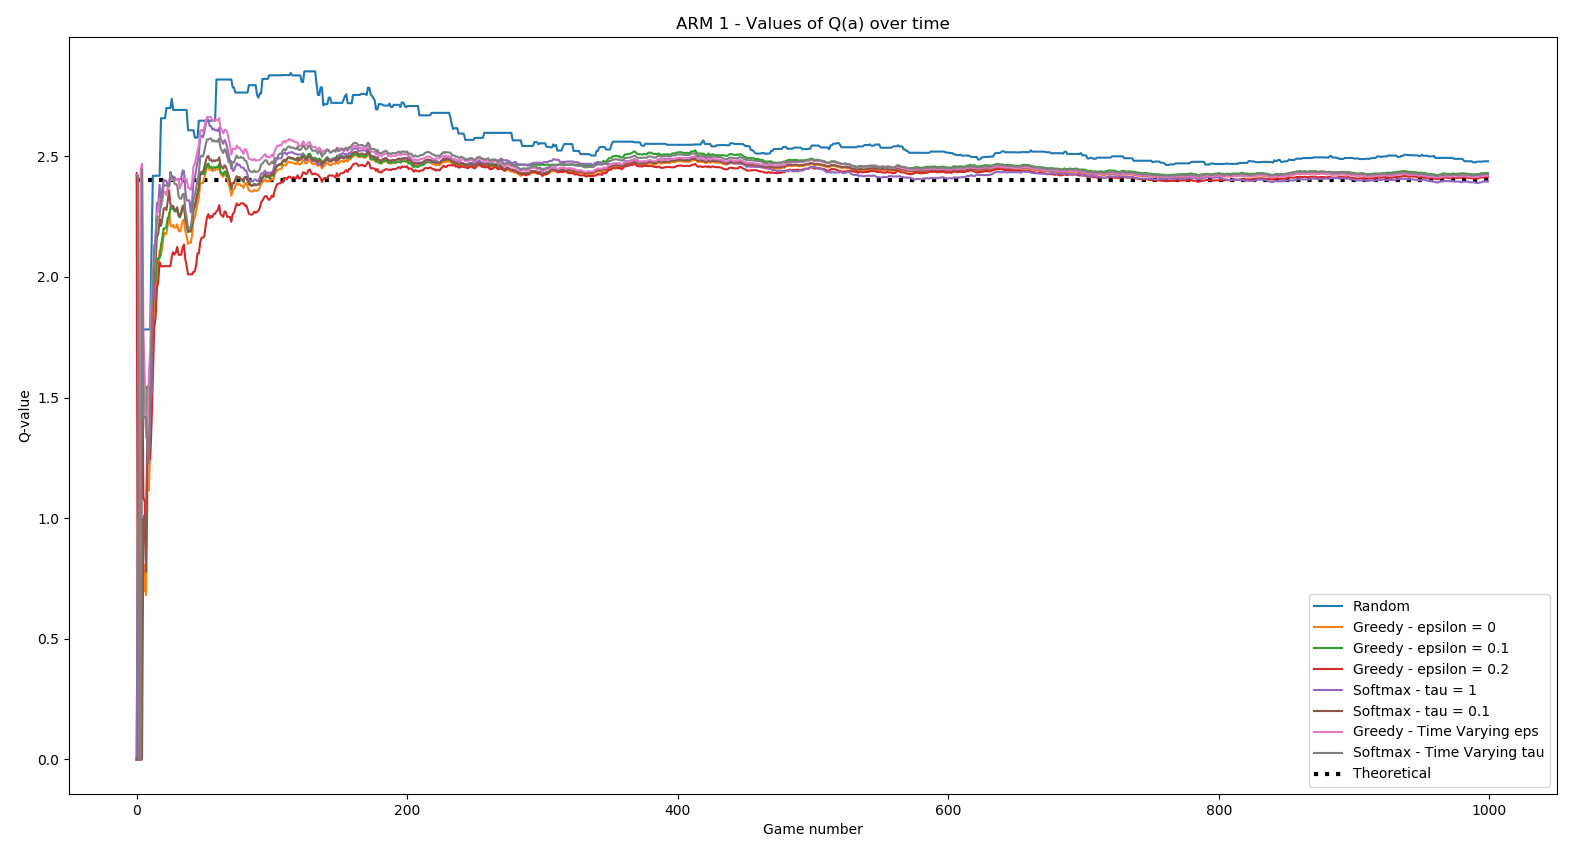
\includegraphics[scale=0.35]{fig/bandit3-arm1.png}
  \caption{Evolution of the Q-value for Arm 1}
  \label{fig:bandit3-arm1}
\end{figure}

\begin{figure}[H]
  \centering
  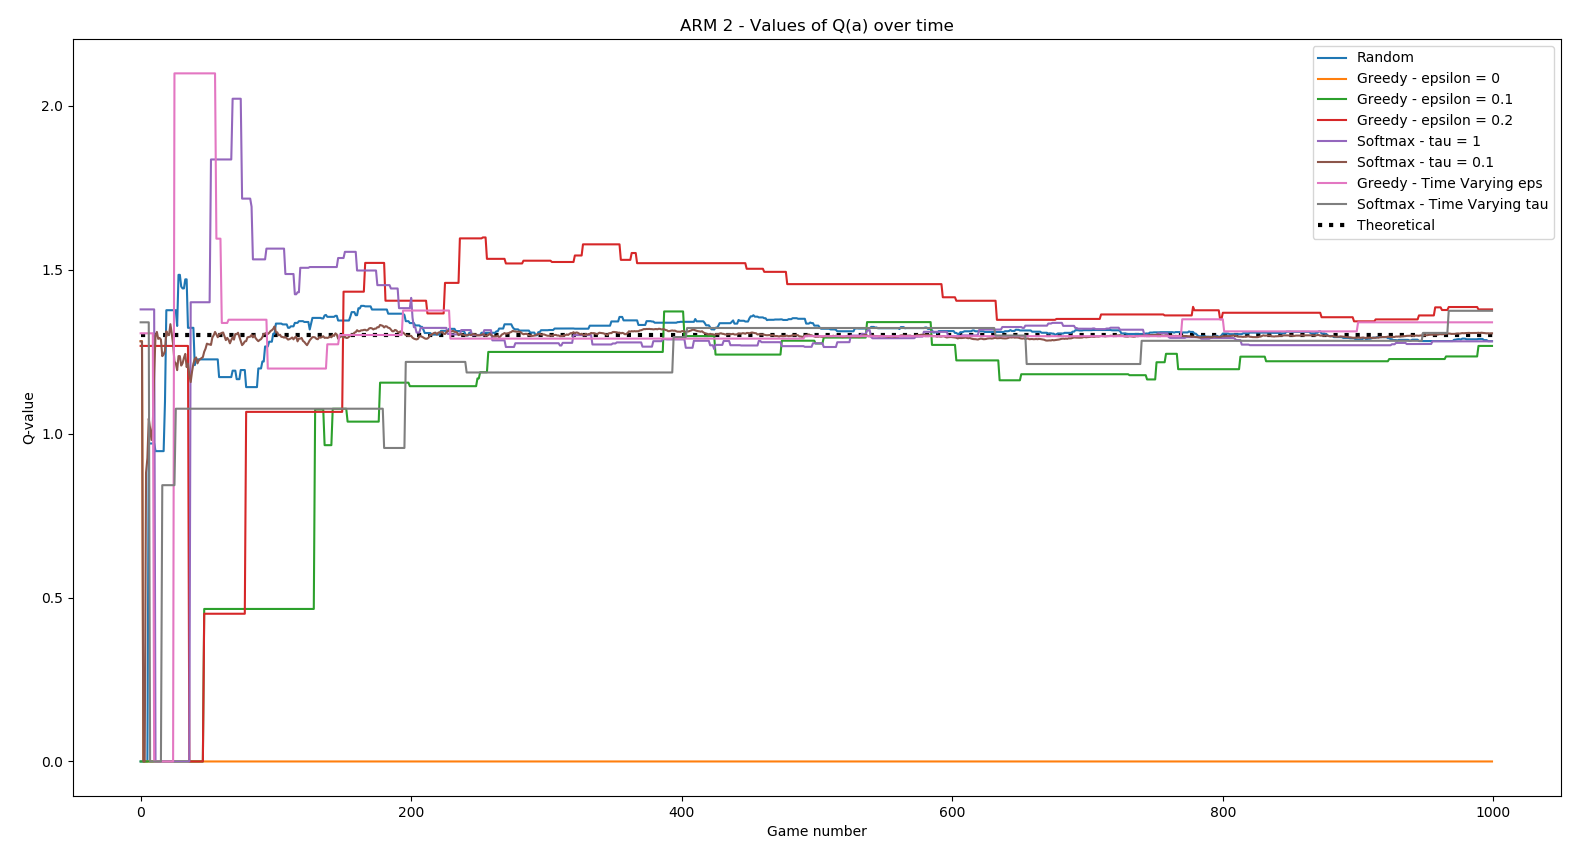
\includegraphics[scale=0.37]{fig/bandit3-arm2.png}
  \caption{Evolution of the Q-value for Arm 2}
  \label{fig:bandit3-arm2}
\end{figure}

\begin{figure}[H]
  \centering
  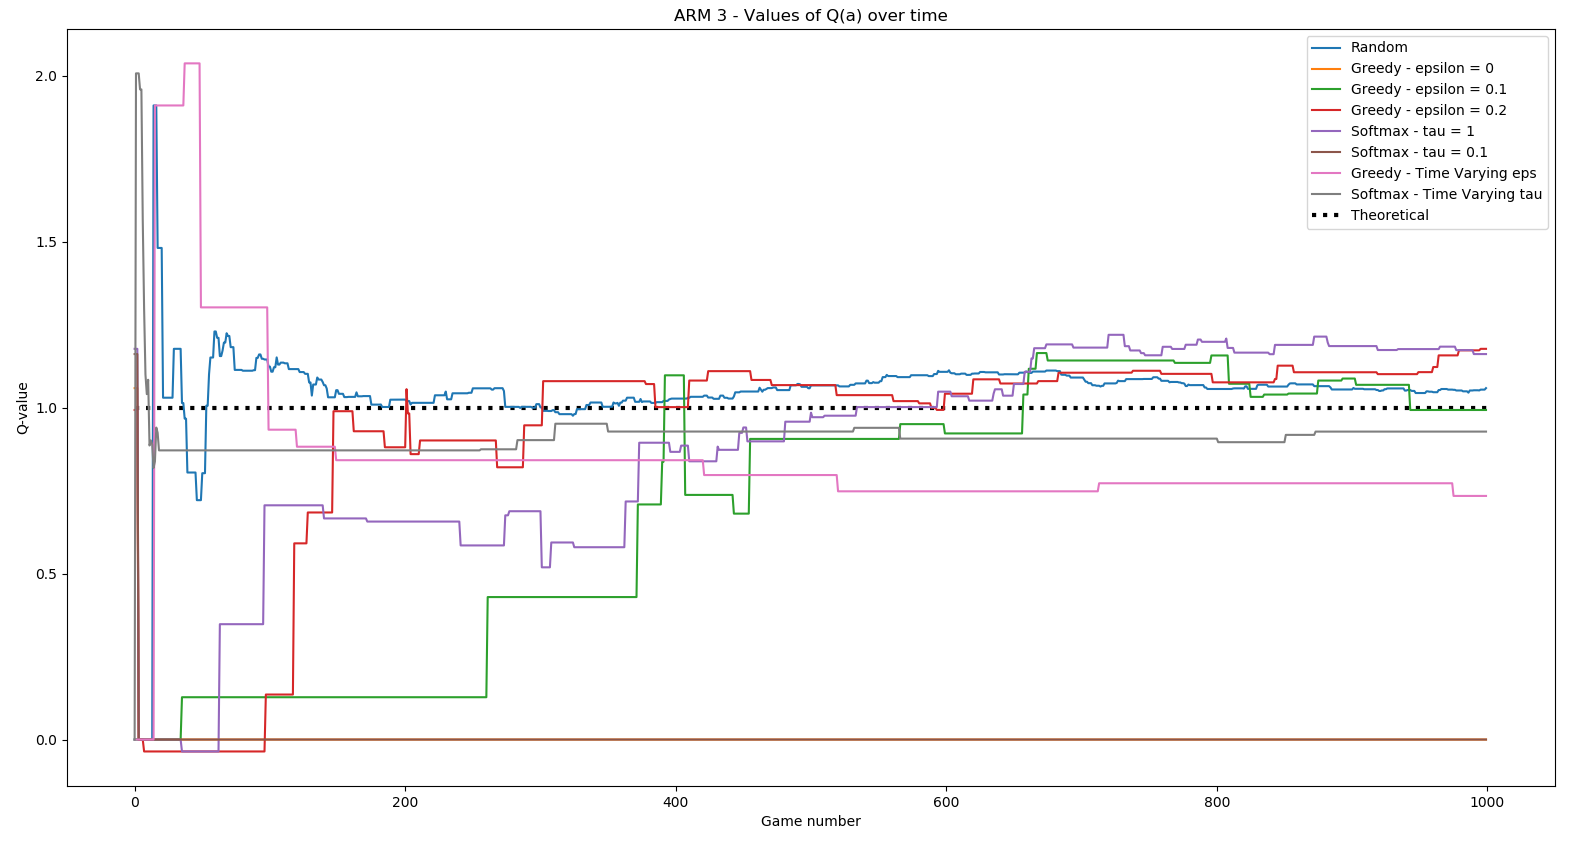
\includegraphics[scale=0.37]{fig/bandit3-arm3.png}
  \caption{Evolution of the Q-value for Arm 3}
  \label{fig:bandit3-arm3}
\end{figure}

\begin{figure}[H]
  \centering
  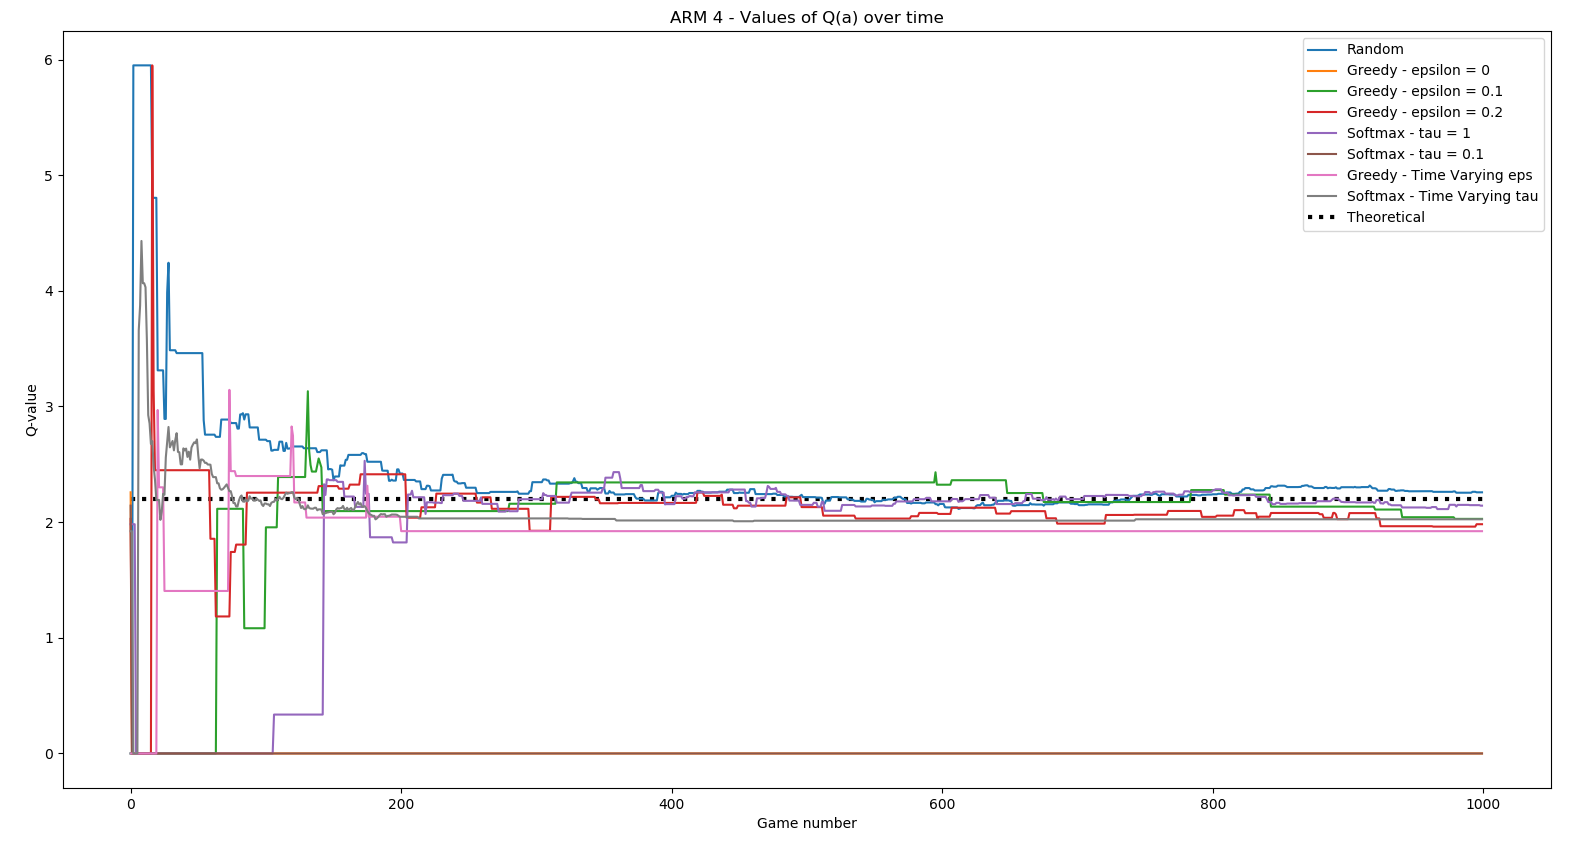
\includegraphics[scale=0.34]{fig/bandit3-arm4.png}
  \caption{Evolution of the Q-value for Arm 4}
  \label{fig:bandit3-arm4}
\end{figure}

\subsubsection{Frequency of each action being selected}

The \autoref{fig:bandit3-counters} is proving that the exploration is more present for the case of Softmax using time varying parameter comapared to a fixed parameter $\tau = 0.1$ where the exploration was null. On the other hand, for the $\epsilon$-greedy with $\epsilon (t)$, it looks like an average of the frequency computed for fixed parameter $\epsilon = 0, 0.1$ and $0.2$ which is normal because in 1000 simulations, the algorithm is covering all the values between 1 and 0.03. Finally, what we can say about these 2 new algorithms is that they are quite good and even looks a bit more robust than the ones with a fixed parameter.  

\begin{figure}[H]
  \centering
  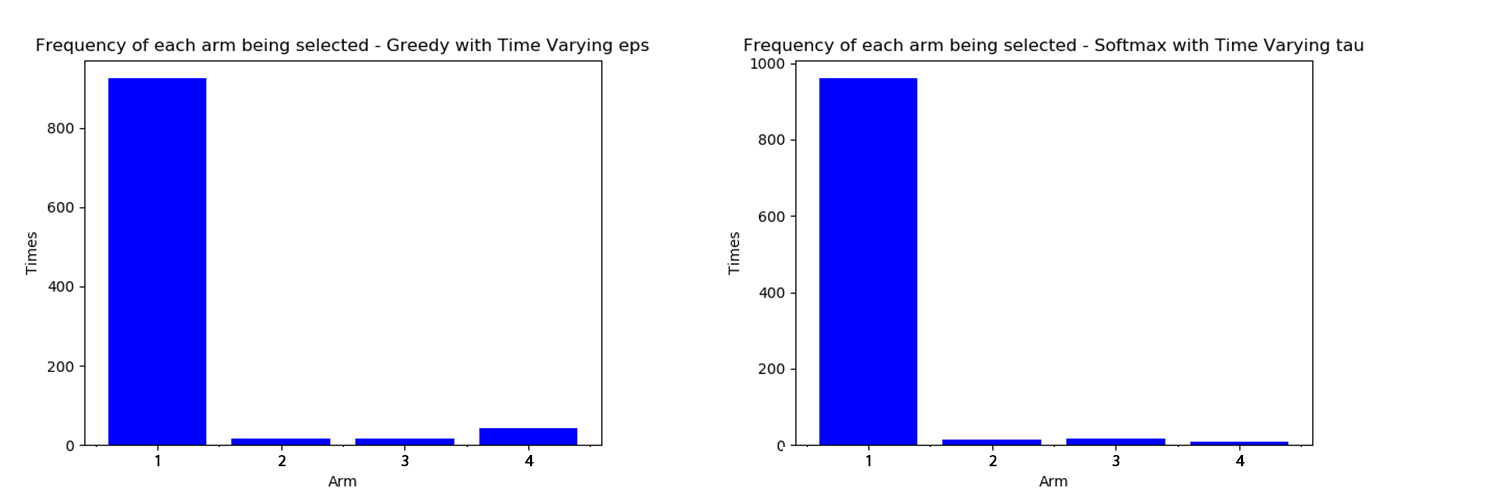
\includegraphics[scale=1.3]{fig/bandit3-counters.png}
  \caption{Frequency of each arm being selected using greedy $\epsilon (t)$ and softmax $\tau (t)$ for 1000 time steps}
  \label{fig:bandit3-counters}
\end{figure}

\subsection{Conclusion}
After observing the results with multiple conditions, what we can conclude is that the best results are obtained with an exploration phase. Chosing an action randomly is never a good solution whether the condition. The softmax and $\epsilon$-greedy algorithms are then the best method to adopt. 

\newpage

\section{Second game: Windy Gridworld}

\subsection{Plot of an execution of Windy Gridworld}

\subsection{Best actions and path taken}

An execution of the $Q$-learning algorithm for the Windy Gridworld problem is presented in the \autoref{fig:grid-path}. In the figure, the start point was $(3,0)$ and the goal point is represented by a red point and is $(9,3)$ in this case. Each cell is showing its best action. The red arrows are representing the path taken to reach the goal. In this run, $\alpha = 0.1$, $\gamma = 0.9$ and $\epsilon = 0.2$. The $Q$-values have been computed over 5000 episodes.   

\begin{figure}[H]
  \centering
  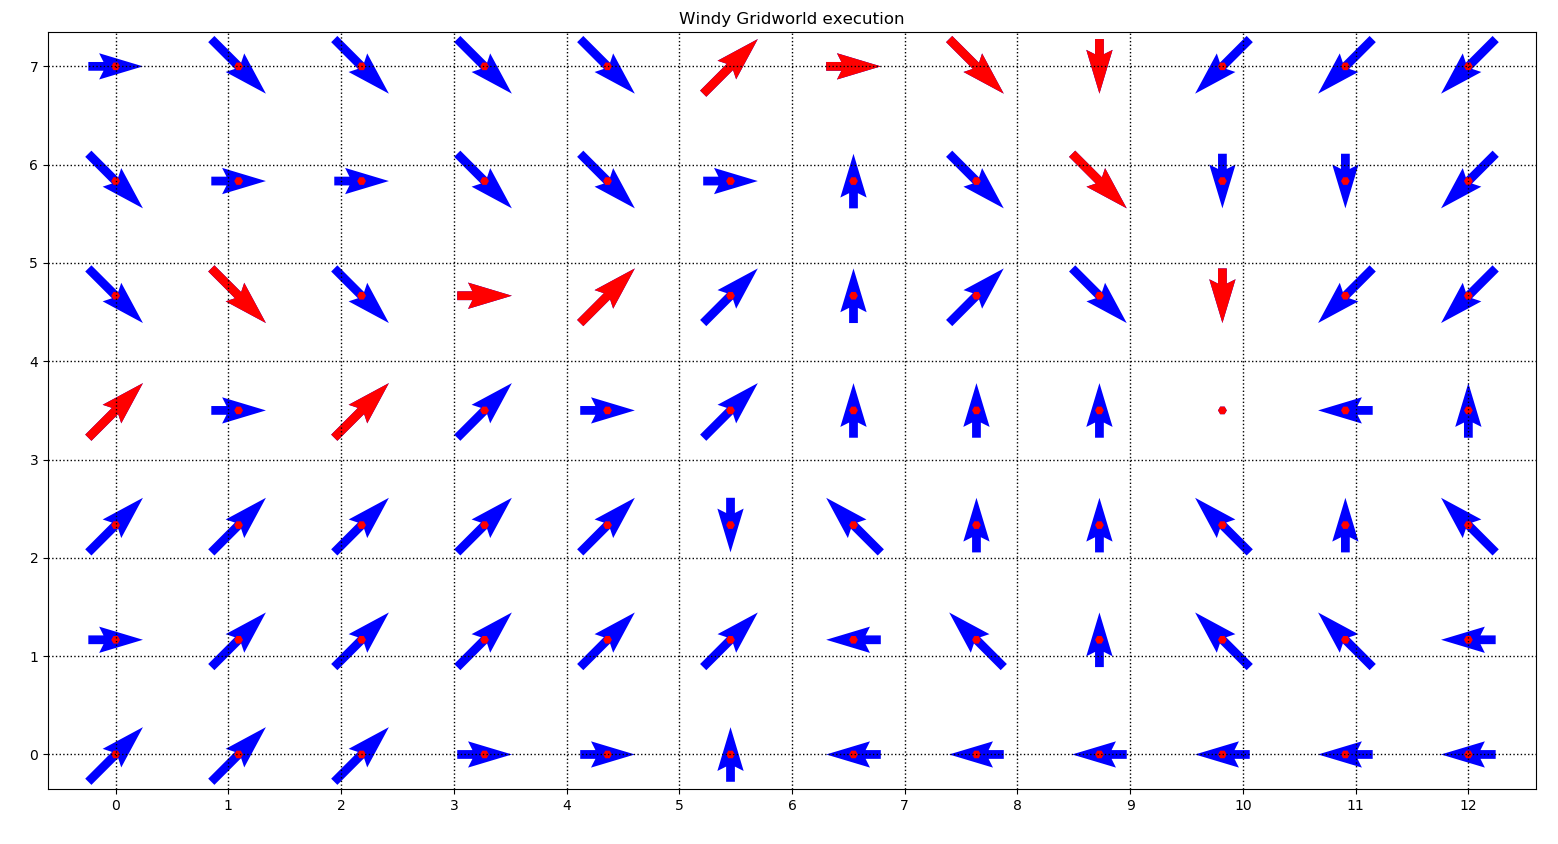
\includegraphics[scale=0.35]{fig/grid-path.png}
  \caption{Execution of Windy Gridworld}
  \label{fig:grid-path}
\end{figure}

\subsubsection{Observation} 
The first observation is that generally all the best actions chosen by each cell is not really accurate, even they are mostly converging to the goal point, we can see that the exploration is kinda weak such that some arrows are completely not pointing the goal even they're beside the goal point. For instance, the arrow left to the goal is pointing to the north while the goal is just one cell to its right. This is explained by the small value chosen for $\epsilon$.   

\subsection{Statistics}
The two statistics that we are interested of are the total collected reward per episode and the number of steps to reach the goal per episode. The first one is presented in the \autoref{fig:grid-totalReward} and the second one in the \autoref{fig:grid-steps}. 

\begin{figure}[H]
  \centering
  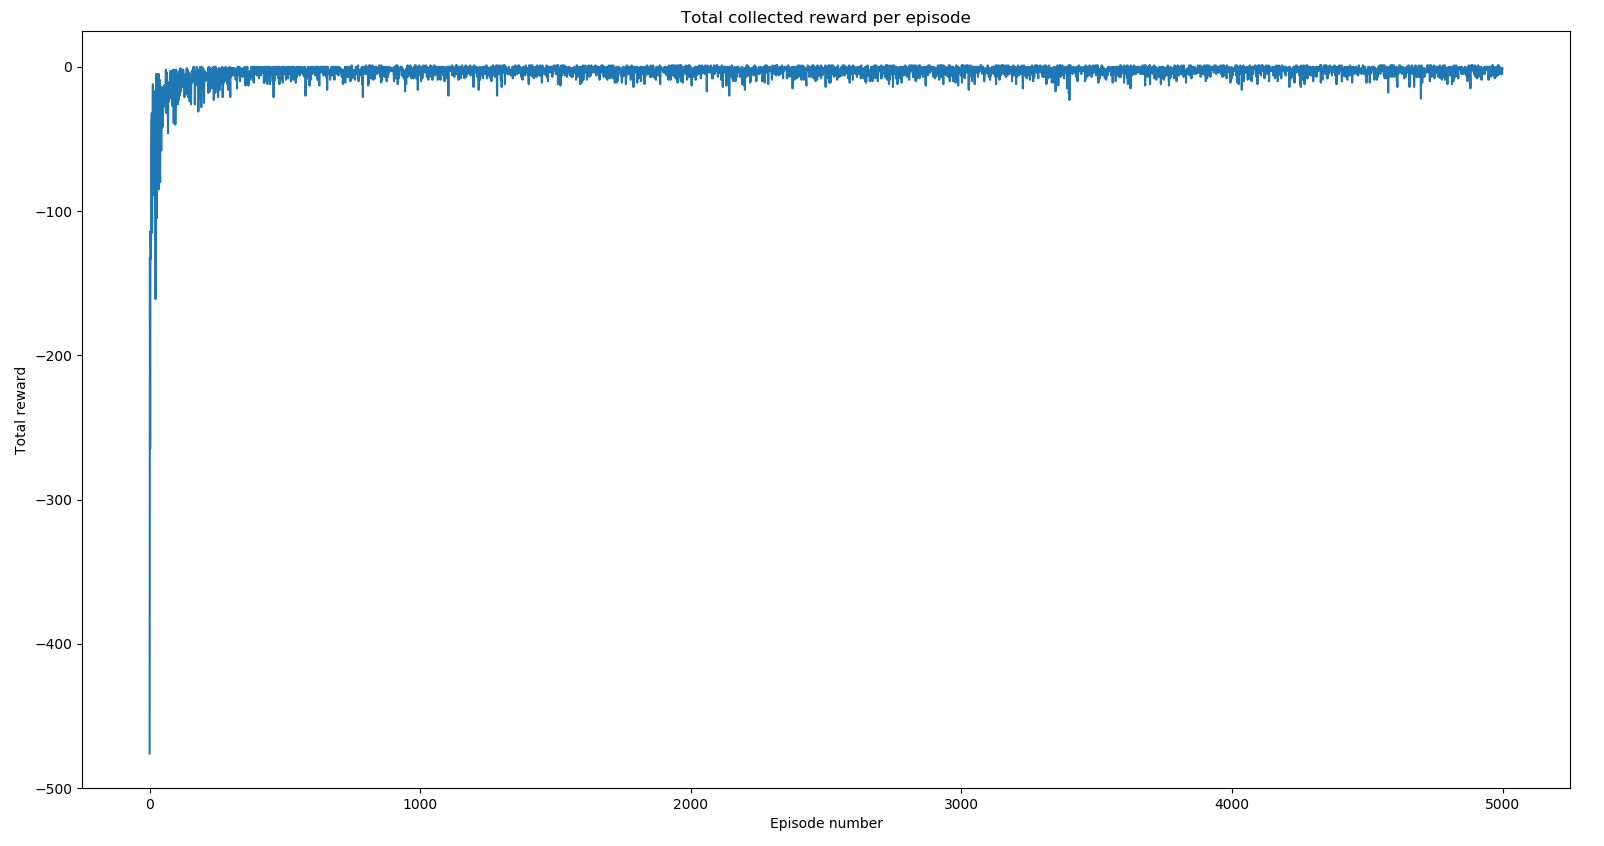
\includegraphics[scale=0.35]{fig/grid-totalReward.png}
  \caption{Total reward per episode}
  \label{fig:grid-totalReward}
\end{figure}

\begin{figure}[H]
  \centering
  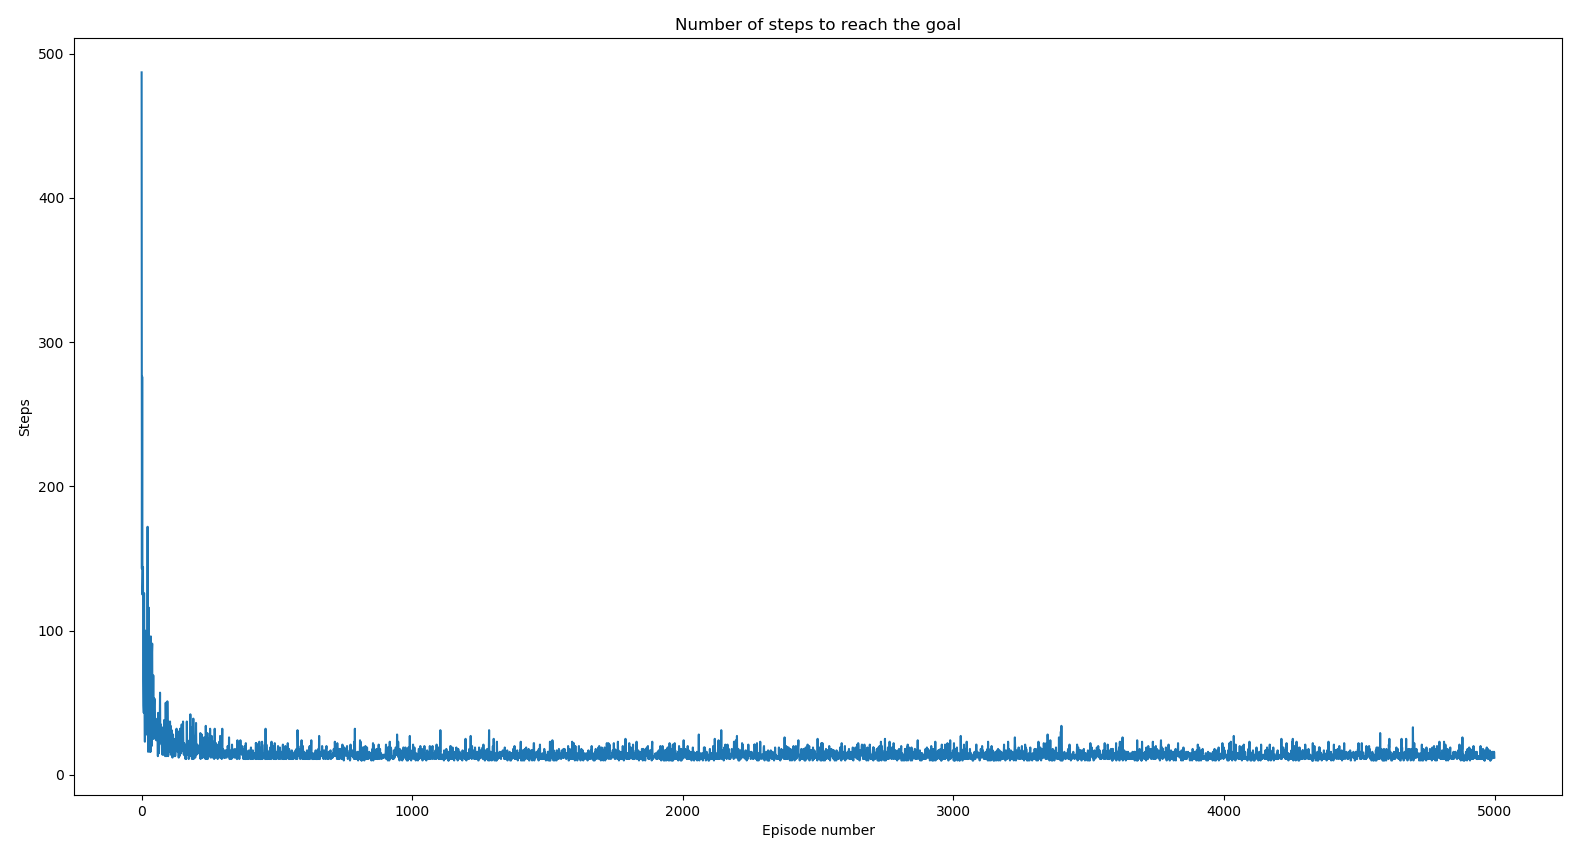
\includegraphics[scale=0.35]{fig/grid-steps.png}
  \caption{Number of steps to reach the goal per episode}
  \label{fig:grid-steps}
\end{figure}

\subsubsection{Observation} 
What we first observe is that the total reward and the number of steps to reach the goal is proportional. Indeed, the first steps are taking a long time to reach the goal (e.g 500 for the first one) and impacts then the total reward because each step is decreasing the reward of 1 while the goal isn't reached (reward is increased by 10 when reached). Nevertheless, the learning done at the beginning seems to be good because after 250-300 episodes the steps number to find the goal is stationary on an average of 15-20 steps.      

\subsection{Question 1: Changing $\epsilon$}

\subsubsection*{Statement}
\textit{How will the learning process change if we make $\epsilon$ = 0, while keeping the other parameters the same?} 

\subsubsection{Result}
As saw in the previous game, $\epsilon$ is representing the rate of exploration. By putting $\epsilon$ to zero, we define that no exploration is done, only exploitation which means that from the beginning to the end, the same action is always picked. However, what we can observe from the results shown in \autoref{fig:grid-eps0} is that some exploration are done at the beginning for 400-500 episodes. In fact, what is happening is that the $\epsilon$-greedy algorithm is always taking the maximum value of $Q(s,a)$. As saw before, when the goal isn't reached, the reward will be negative. Thereby, by initializing the $Q$-values to all zeros, the $\epsilon$-greedy algorithm will pick randomly an action which its $Q$-value equals zero. The exploration will end when all the actions have been explored once. At this time, the maximum $Q$-value will be the same for every other rounds.  

\begin{figure}[H]
  \centering
  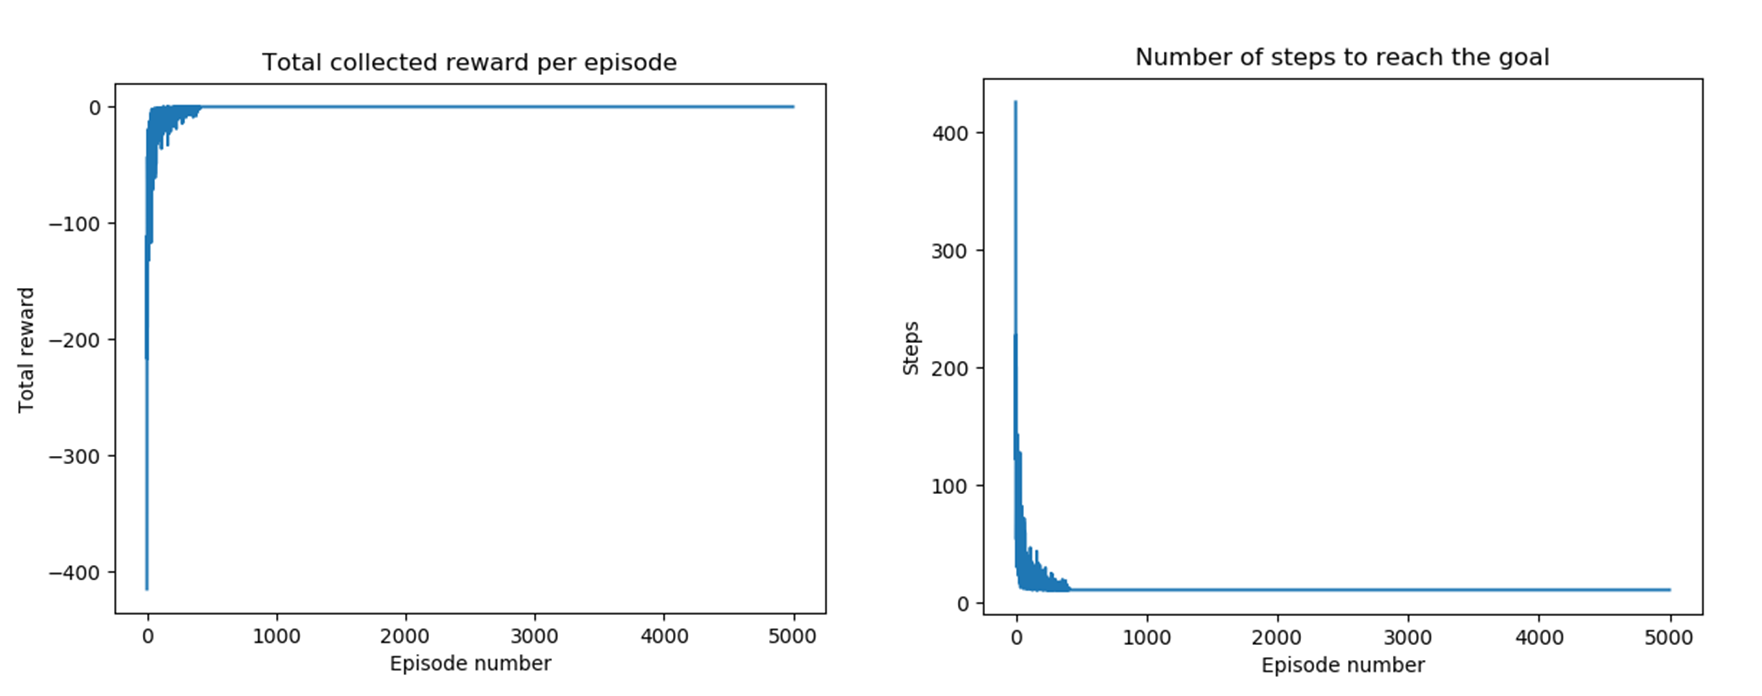
\includegraphics[scale=0.25]{fig/grid-eps0.png}
  \caption{Results with $\epsilon = 0$}
  \label{fig:grid-eps0}
\end{figure}

\subsection{Question 2: Changing $\gamma$}

\subsubsection*{Statement}
\textit{How will the learning process change if we make $\gamma$ = 1, while keeping the other parameters the same?} 

\subsubsection{Result}
$\gamma$ is the discount factor which means that $\gamma$ is valuing rewards received earlier higher than those received later (reflecting the value of a "good start"). By putting $\gamma$ to 1, it means that the future values will have the same impact weight than the first received values. The learning is then taking in account fairly the current and the future values. 

\newpage
\section{Third game: Graphical Coordination Game}

\subsection{Payoff matrix}
First of all, let's have a look on the payoff matrix considering 2 and 3 actions. The reward for each player is symmetric. Indeed, an agent is rewarded only if the other player plays the same action than him, otherwise whether the action played, if the other agent plays another action, the payoff of both player will be zero. In other words, the agents have to be coordinated to win. 

\begin{table}[H]
\begin{minipage}{.5\linewidth}
\centering
\begin{tabular}{|c|c|c|}
  \hline
  	 \backslashbox[0pt][l]{Agent 1}{Agent 2}       & Action 1 & Action 2 \\
  \hline
  	Action 1 & 1 & 0 \\
  \hline
  Action 2   & 0 &  1\\
  \hline
\end{tabular}
\end{minipage}
\begin{minipage}{.5\linewidth}
\centering
\begin{tabular}{|c|c|c|c|}
  \hline
  	   \backslashbox[0pt][l]{Agent 1}{Agent 2}      & Action 1 & Action 2 & Action 3 \\
  \hline
  	Action 1 & 1 & 0 & 0\\
  \hline
  Action 2   & 0 &  1 & 0\\
  \hline
   Action 3   & 0 &  0 & 1\\
  \hline
\end{tabular}
\end{minipage}
\caption{Payoff matrices for 2 and 3 actions game}
\end{table}

\subsection{Convergence time}
% pour 2: [50000, 8664.92039800995, 4566.87, 3780.26, 2485.685, 2173.13, 2026.595, 2098.34, 2265.085, 3329.99]

% Pour 3: [50000, 11936.940594059406, 5201.59, 3601.425, 3208.995, 2787.81, 2326.38, 2270.1, 2625.88, 3713.315] 
The average value of the convergence time according to the value of $\alpha$ is given in \autoref{tab:convergence-alpha-2} for 2 actions and \autoref{tab:convergence-alpha-3} for 3 actions. Note that we use arbitrary 50000 as value of $T_{max}$ which means that it never converges when exceeding this threshold value. Thereby, in the \autoref{fig:coord-convergenceAlpha}, an average convergence time of 50000 means a non-converging game for this $\alpha$ value. The \autoref{fig:coord-convergenceAlpha-bis} shows the same graph as \autoref{fig:coord-convergenceAlpha} without the non-converging $\alpha$. 

\vspace{3cm}

\begin{table}[H]
\begin{minipage}{.5\linewidth}
\centering
\begin{tabular}{|c|c|} 
 \hline
  $\alpha$ & Convergence time (average) \\
  \hline
  0 & Never converge \\
  0.1 & 8664 \\
  0.2 & 4566 \\
  0.3 & 3780 \\
  0.4 & 2485 \\
  0.5 & 2173 \\
  0.6 & 2026 \\
  0.7 & 2098 \\
  0.8 & 2265 \\
  0.9 & 3329 \\
  1 & Never converge \\
  \hline
\end{tabular}
\caption{Average convergence time for 2 actions} \label{tab:convergence-alpha-2}
\end{minipage}
\begin{minipage}{.5\linewidth}
\centering
\begin{tabular}{|c|c|} 
 \hline
  $\alpha$ & Convergence time (average) \\
  \hline
  0 & Never converge \\
  0.1 & 11936 \\
  0.2 & 5201 \\
  0.3 & 3601 \\
  0.4 & 3208 \\
  0.5 & 2787 \\
  0.6 & 2326 \\
  0.7 & 2270 \\
  0.8 & 2625 \\
  0.9 & 3713 \\
  1 & Never converge \\
  \hline
\end{tabular}
\caption{Average convergence time for 3 actions} \label{tab:convergence-alpha-3}
\end{minipage}
\end{table}


\begin{figure}[H]
  \centering
  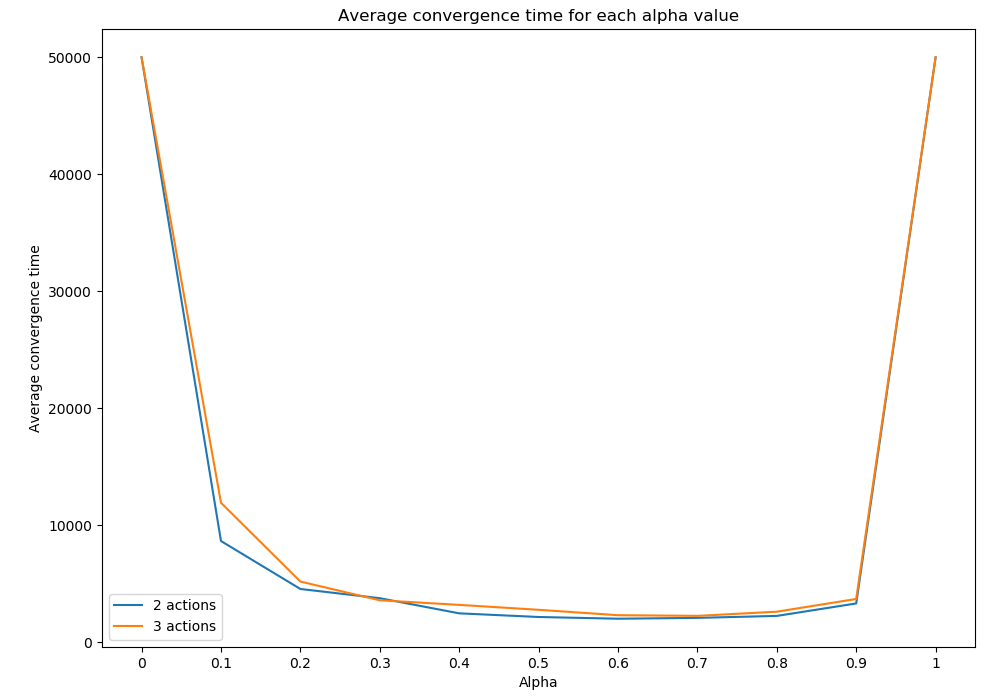
\includegraphics[scale=0.36]{fig/coord-convergenceAlpha.png}
  \caption{Average convergence time for each $\alpha$ value}
  \label{fig:coord-convergenceAlpha}
\end{figure}

\begin{figure}[H]
  \centering
  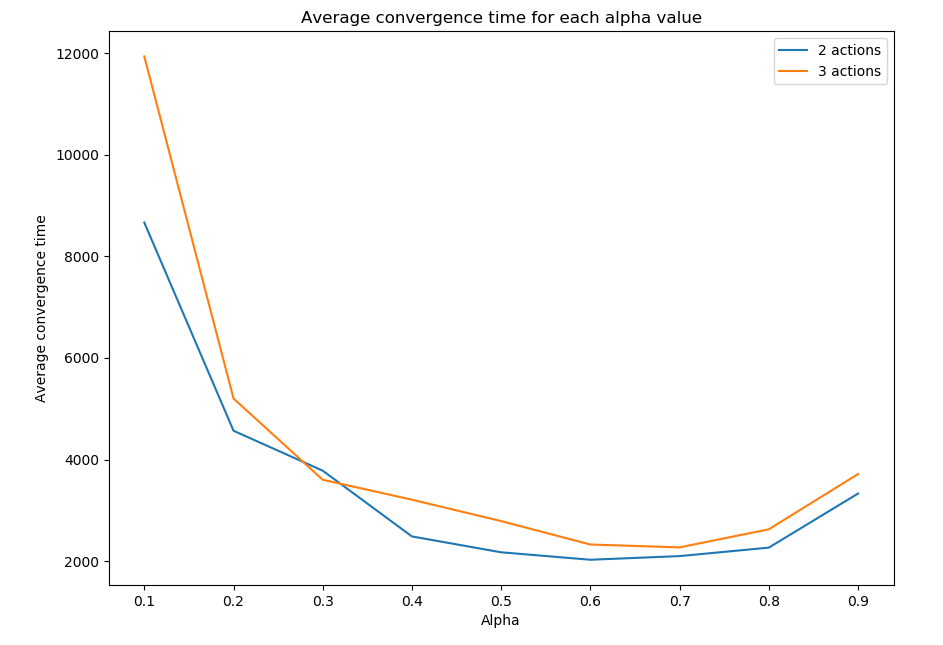
\includegraphics[scale=0.41]{fig/coord-convergenceAlpha-bis.png}
  \caption{Average convergence time for converging $\alpha$ value}
  \label{fig:coord-convergenceAlpha-bis}
\end{figure}


\subsubsection{What is the role of $\alpha$ for the Win-Stay-Lose-probabilistic-Shift algorithm?} 

The $\alpha$ is the lose-probabilistic-shift. The action change depends of this value of $\alpha$. An agent will keep his action with a probability of 1-$\alpha$. A small value of $\alpha$ means that an agent is flexible and will change quite often his action while a large value of $\alpha$ means that the agent will mostly keep playing his action. 

\subsubsection{How is the convergence time affected by the value of $\alpha$?} 
As \autoref{fig:coord-convergenceAlpha-bis} shows, if $\alpha$? is too small, the agents will really often change their actions in every round which means that the actions of the agents keep changing. Getting coordinated becomes then more difficult. From $\alpha = 0.5$ to $\alpha = 0.8$, it becomes really fast to get the coordinated state (around 2000 rounds).   

\subsubsection{Which $\alpha$ value(s) result in the fastest convergence time for your setting?}
Generally, the fastest convergence will be between $\alpha = 0.5$ and $\alpha = 0.8$. In this interval, the probability to change action is not to big and not to small. These values are then ideal to get the convergence quickly. 

\subsubsection{For which $\alpha$ values the algorithm fails to converge?}
It exists 2 values of $\alpha$ which the algorithm will always fail to converge : $\alpha = 0$ and $\alpha = 1$. It is logic because in the first case ($\alpha = 0$), the agents will change their action in every round which means that if their basic configuration isn't respecting the convention, i.e the same action for every agent, it becomes impossible to get this convergence. Same logic for $\alpha = 1$ which means that the agents will never change their action. The only case where it converges is that the random action choice at first round is the same for every agent. At this time, it will converges immediately after 10 iterations. Nevertheless, this case is somehow impossible with that number of agents or really rare. 

\subsubsection{How is the convergence time affected by the number of actions?}
Obviously, less is the number of actions, less the convergence time will be. It is a simple combinatoric problem which shows that exists more combination with more actions, thus it exists more possibilities when assigning a random action to each agent. Indeed, the numbers of combinations is : 

$$ C_{n}^{k} = {n \choose k} = \frac{n!}{(n-k)! \cdot k!}$$
 
\noindent
where $n$ is the number of actions and $k$ the number of agents. \\

\noindent
For 26 agents, it means that for 2 actions, it exists 325 combinations possible for the assignment of actions in the first iterations and 2600 for 3 actions. Thus, this difference is mostly marked for the first iterations but will of course also impact the sequel of iterations. 
 
\end{document}